%_____________________________________________________________________________
%=============================================================================
% main.tex v6 (10-11-2013) \ldots dibuat oleh Lionov - Informatika FTIS UNPAR
% 
% Ini adalah file utama (main.tex), berisi perintah-perintah yang khusus 
% dibuat untuk template ini
%
% 			JANGAN MENGUBAH APAPUN DI DALAM FILE INI,
%			KECUALI ANDA TAHU APA YANG ANDA LAKUKAN !!!
%
% Jika ada tambahan perintah, dapat anda tuliskan di tempat yang telah disediakan 
% di baris 295 pada file ini
% Jika daftar tabel tidak digunakan, anda harus menghapus (beri komentar) secara
% manual di baris 470
%
% Bug, kritik, saran: silahkan kirimkan via email ke lionov@unpar.ac.id
%
% Perubahan pada versi 6 (10-11-2013):
%	- perbaikan pada abstract dengan pngaragraf lebih dari satu: perbaikan vertical spacing
%	- perbaikan pada tampilan bab dan lampiran: tidak perlu menuliskan apapun untuk 
%	  menampilkan semuanya (di data.tex) atau -1 jika tidak ada lampiran
%	- halaman bernomor genap untuk halaman romawi sudah dimunculkan
%	- Kurikulum 2013 : perubahan nama buku skripsi 
%
% Perubahan dari versi sebelumnya :
%	versi 5 (21-10-2012)
%	- halaman terakhir setiap bab tidak ada headernya jika kosong
%	versi 4 (06-08-2012)
% 	- penggabungan main.tex, depan.tex dan setup.tex menjadi main.tex
% 	- menambahkan keterangan di lampiran untuk kode program 
% 	- ukuran font dapat diubah langsung di tiap lampiran
% 	versi 3 (09-07-2012): 
%	- Tidak ada di file ini
% 	versi 2 :
% 	- "Daftar Referensi" tidak perlu diubah secara manual (tidak perlu mengubah file bahasai.ldf)
% 	- Bahasa Indonesia dari abstract adalah abstrak (secara otomatis), bukan ringkasan
% 	- Spasi pada buku dokumen final adalah onehalfspacing
%
% to do : - hilangkan secara otomatis daftar tabel/gambar jika tidak digunakan
%         - (IT) aturan penulisan algoritma untuk IT (pakai algo.sty ?)
%=============================================================================

%=============================================================================
% setup.tex v2 (08-07-2012)
% Perubahan pada versi 2:
% - Menambahkan perintah untuk judulINA dan judulENG
% - Menghapus \usepackage{microtype}, yang pada beberapa kasus menjadi masalah
%=============================================================================
% depan.tex v2 (09-07-2012)
% Perubahan pada versi 2:
% - Menambahkan halaman depan dalam bahasa inggris
%=============================================================================

%setup.tex
\documentclass[11pt,a4paper,twoside,openright,notitlepage]{report} 

\usepackage[bahasa]{babel} %bahasa indonesia
\usepackage[T1]{fontenc}  %encoding
% \usepackage{mathptmx}
% \usepackage{venturisold}
% \usepackage{helvet}
% \usepackage{fouriernc} 
\usepackage{abstract} %manipulasi abstract
\usepackage{chappg} % format daftar isi 
\usepackage{color} %warna
\usepackage{etoolbox} %untuk programming if-then
\usepackage{fancyhdr} %format header & footer
\usepackage{float} %penempatan gambar di tempat yg seharusnya
\usepackage[inner=2.5cm,outer=2cm,top=2.5cm,bottom=2.5cm]{geometry} %margin
\usepackage{graphicx} %gambar
\usepackage{listings} %source code
\usepackage{lscape} %landscape untuk source code
\usepackage{multicol} %multiple column
\usepackage{ifthen} % if then
\usepackage[pagewise]{lineno} %line numbering
\usepackage{lipsum} % untuk testing
\usepackage{titlesec} %judul header
\usepackage{tocbibind} %daftar isi, gambar, tabel dll
\usepackage{tocloft} % format daftar isi 
\usepackage{setspace} %line spacing
\usepackage{xstring} %manipulasi string
\usepackage[plainpages=false,pdfpagelabels,unicode]{hyperref} %\autoref, \phantomsection & link 

\usepackage{emptypage}

\let\abstractname\Abstrak

\titleformat{\chapter}[display] {\Large\bfseries\centering}{\MakeUppercase{\chaptertitlename} \thechapter}{15pt}{\Large\MakeUppercase}

\renewcommand{\cftchapfont}{\scshape \bfseries}

\renewcommand{\cfttoctitlefont}{\hfill\Large\bfseries\MakeUppercase}
\renewcommand{\cftaftertoctitle}{\hfill}
\renewcommand{\cftloftitlefont}{\hfill\Large\bfseries\MakeUppercase}
\renewcommand{\cftafterloftitle}{\hfill}
\renewcommand{\cftlottitlefont}{\hfill\Large\bfseries\MakeUppercase}
\renewcommand{\cftafterlottitle}{\hfill}

% Tidak perlu ada kata "Bab", "Gambar" atau "Tabel" di daftar 
% \renewcommand{\cftchappresnum}{{\bf \scshape Bab} } 
% \renewcommand{\cftchapnumwidth}{1.5cm}
% \renewcommand{\cftfigpresnum}{{Gambar\ }} 
% \renewcommand{\cftfignumwidth}{2.5cm}
% \renewcommand{\cfttabpresnum}{{Tabel\ }} 
% \renewcommand{\cfttabnumwidth}{2cm}

\newcommand{\apptoc}{
	% Hapus kata "Lampiran" dari daftar isi
	%\addtocontents{toc}{\protect\renewcommand{\protect\cftchappresnum}{\bf \scshape Lampiran\  }}%
	%\addtocontents{toc}{\protect\renewcommand{\protect\cftchapnumwidth}{2.75cm}}
	\addtocontents{toc}{\protect\renewcommand{\protect\cftchappresnum}{\bf \scshape}}%	

}

\newcommand{\vnama}{Jane Doe}
\newcommand{\vlnama}{John Doe}
\newcommand{\vnpm}{1992700001}
\newcommand{\vprodiINA}{SAINS}
\newcommand{\vprodiENG}{SCIENCE}
\newcommand{\vstaINA}{UJIAN}
\newcommand{\vstaENG}{EXAM}
%\newcommand{\vjudul}{Judul Skripsi/Tugas Akhir}
\newcommand{\vpembu}{Plato}
\newcommand{\vpembs}{Euclid}
\newcommand{\vpengi}{Plato}
\newcommand{\vpengii}{Euclid}
\newcommand{\vtanggal}{1}
\newcommand{\vbulan}{Januari}
\newcommand{\vtahun}{1970}
\newcommand{\vmode}{final}
\newcommand{\vspacing}{double}
\newcommand{\vlineno}{yes}
\newcommand{\vkunciina}{Skripsi, Tugas Akhir}
\newcommand{\vkuncieng}{Undergraduate Thesis, Final Project}
\newcommand{\vkajur}{Jack Doe}
\newcommand{\vkajurmat}{Jack Doe}
\newcommand{\vkajurfis}{Jack Doe}
\newcommand{\vkajurtif}{Jack Doe}

\newcommand{\namanpm}[2]{
	\renewcommand{\vnama}{\uppercase{#1}} \renewcommand{\vlnama}{#1} \hypersetup{pdfauthor={#2 - #1}}
	\renewcommand{\vnpm}{#2} \hypersetup{pdfcreator={#2}} \StrChar{\vnpm}{6}[\vprodiN]
	\ifdefstring{\vprodiN}{1}{
		\renewcommand{\vprodiINA}{MATEMATIKA} \renewcommand{\vprodiENG}{MATHEMATICS} 
		\renewcommand{\vstaINA}{SKRIPSI} \renewcommand{\vstaENG}{FINAL PROJECT} \renewcommand{\vkajur}{\vkajurmat}}{}
	\ifdefstring{\vprodiN}{2}{
		\renewcommand{\vprodiINA}{FISIKA} \renewcommand{\vprodiENG}{PHYSICS} 
		\renewcommand{\vstaINA}{TUGAS AKHIR} \renewcommand{\vstaENG}{FINAL PROJECT} \renewcommand{\vkajur}{\vkajurfis}}{}
	\ifdefstring{\vprodiN}{3}{
		\renewcommand{\vprodiINA}{TEKNIK INFORMATIKA} \renewcommand{\vprodiENG}{INFORMATICS} 
		\renewcommand{\vstaINA}{SKRIPSI} \renewcommand{\vstaENG}{UNDERGRADUATE THESIS} \renewcommand{\vkajur}{\vkajurtif}}{}}

%\newcommand{\judul}[1]{\renewcommand{\vjudul}{\uppercase{#1}}\hypersetup{pdftitle={#1}, pdfsubject={#1}}}
\newcommand{\pembimbing}[2]{\renewcommand{\vpembu}{#1}\renewcommand{\vpembs}{#2}}
\newcommand{\penguji}[2]{\renewcommand{\vpengi}{#1}\renewcommand{\vpengii}{#2}}
\newcommand{\kajur}[3]{\renewcommand{\vkajurmat}{#1}\renewcommand{\vkajurfis}{#2}\renewcommand{\vkajurtif}{#3}}
\newcommand{\tanggal}[3]{\renewcommand{\vtanggal}{#1}\renewcommand{\vtahun}{#3}
	\newcommand{\vcbulan}{#2}
	\ifdefstring{\vcbulan}{1}{\renewcommand{\vbulan}{Januari}}{}
	\ifdefstring{\vcbulan}{2}{\renewcommand{\vbulan}{Februari}}{}
	\ifdefstring{\vcbulan}{3}{\renewcommand{\vbulan}{Maret}}{}
	\ifdefstring{\vcbulan}{4}{\renewcommand{\vbulan}{April}}{}
	\ifdefstring{\vcbulan}{5}{\renewcommand{\vbulan}{Mei}}{}
	\ifdefstring{\vcbulan}{6}{\renewcommand{\vbulan}{Juni}}{}
	\ifdefstring{\vcbulan}{7}{\renewcommand{\vbulan}{Juli}}{}
	\ifdefstring{\vcbulan}{8}{\renewcommand{\vbulan}{Agustus}}{}
	\ifdefstring{\vcbulan}{9}{\renewcommand{\vbulan}{September}}{}
	\ifdefstring{\vcbulan}{10}{\renewcommand{\vbulan}{Oktober}}{}
	\ifdefstring{\vcbulan}{11}{\renewcommand{\vbulan}{November}}{}
	\ifdefstring{\vcbulan}{12}{\renewcommand{\vbulan}{Desember}}{}	
}

\newcommand{\judulINA}[1]{\newcommand{\vjudulINA}{\uppercase{#1}}\hypersetup{pdftitle={#1},pdfsubject={#1}}}
\newcommand{\judulENG}[1]{\newcommand{\vjudulENG}{\uppercase{#1}}\hypersetup{pdftitle={#1},pdfsubject={#1}}}
\newcommand{\abstrakINA}[1]{\newcommand{\vabstrakina}{#1}}
\newcommand{\abstrakENG}[1]{\newcommand{\vabstrakeng}{#1}}
\newcommand{\kunciINA}[1]{\renewcommand{\vkunciina}{#1} \hypersetup{pdfkeywords={#1}}}
\newcommand{\kunciENG}[1]{\renewcommand{\vkuncieng}{#1}}
\newcommand{\untuk}[1]{\newcommand{\vuntuk}{#1}}
\newcommand{\prakata}[1]{\newcommand{\vprakata}{#1}}
\newcommand{\mode}[1]{\renewcommand{\vmode}{#1}}
\newcommand{\linespacing}[1]{\renewcommand{\vspacing}{#1}}
\newcommand{\linenumber}[1]{\renewcommand{\vlineno}{#1}}

\newcommand{\bab}[1]{\newcommand{\vbab}{#1}}
\newcommand{\lampiran}[1]{\renewcommand{\vlmp}{#1}}

\newcommand{\vpilbab}{0}
\newcommand{\vbaba}{0}\newcommand{\vbabb}{0}\newcommand{\vbabc}{0}
\newcommand{\vbabd}{0}\newcommand{\vbabe}{0}\newcommand{\vbabf}{0}
\newcommand{\vbabg}{0}\newcommand{\vbabh}{0}\newcommand{\vbabi}{0}
\newcommand{\vpillmp}{0}
\newcommand{\vlmpa}{0}\newcommand{\vlmpb}{0}\newcommand{\vlmpc}{0}
\newcommand{\vlmpd}{0}\newcommand{\vlmpe}{0}\newcommand{\vlmpf}{0}
\newcommand{\vlmpg}{0}\newcommand{\vlmph}{0}\newcommand{\vlmpi}{0}
\newcommand{\vlmp}{x}

%	\ifdefempty{#1}{\bab{1,2,3,4,5,6,7,8,9} \tampilbab{\vbab}}{
\newcommand{\tampilbab}[1]{
	\ifdefempty{#1}{
		\renewcommand{\vbaba}{1}\renewcommand{\vbabb}{1}\renewcommand{\vbabc}{1}
		\renewcommand{\vbabd}{1}\renewcommand{\vbabe}{1}\renewcommand{\vbabf}{1}
		\renewcommand{\vbabg}{1}\renewcommand{\vbabh}{1}\renewcommand{\vbabi}{1}}{
	\renewcommand{\do}[1]{
		\renewcommand{\vpilbab}{##1}
		\ifdefstring{\vpilbab}{1}{\renewcommand{\vbaba}{1}}{}
		\ifdefstring{\vpilbab}{2}{\renewcommand{\vbabb}{1}}{}
		\ifdefstring{\vpilbab}{3}{\renewcommand{\vbabc}{1}}{}
		\ifdefstring{\vpilbab}{4}{\renewcommand{\vbabd}{1}}{}
		\ifdefstring{\vpilbab}{5}{\renewcommand{\vbabe}{1}}{}
		\ifdefstring{\vpilbab}{6}{\renewcommand{\vbabf}{1}}{}
		\ifdefstring{\vpilbab}{7}{\renewcommand{\vbabg}{1}}{}
		\ifdefstring{\vpilbab}{8}{\renewcommand{\vbabh}{1}}{}
		\ifdefstring{\vpilbab}{9}{\renewcommand{\vbabi}{1}}{}
	}
	\expandafter\docsvlist\expandafter{#1}
	}
}

\newcommand{\tampillmp}[1]{
	\ifdefempty{#1}{
		\renewcommand{\vlmpa}{1}\renewcommand{\vlmpb}{1}\renewcommand{\vlmpc}{1}
		\renewcommand{\vlmpd}{1}\renewcommand{\vlmpe}{1}\renewcommand{\vlmpf}{1}
		\renewcommand{\vlmpg}{1}\renewcommand{\vlmph}{1}\renewcommand{\vlmpi}{1}}{
	\ifdefstring{#1}{-1}{ }{
		\renewcommand{\do}[1]{ 
			\renewcommand{\vpillmp}{##1}
			\ifdefstring{\vpillmp}{A}{\renewcommand{\vlmpa}{1}}{}
			\ifdefstring{\vpillmp}{B}{\renewcommand{\vlmpb}{1}}{}
			\ifdefstring{\vpillmp}{C}{\renewcommand{\vlmpc}{1}}{}
			\ifdefstring{\vpillmp}{D}{\renewcommand{\vlmpd}{1}}{}
			\ifdefstring{\vpillmp}{E}{\renewcommand{\vlmpe}{1}}{}
			\ifdefstring{\vpillmp}{F}{\renewcommand{\vlmpf}{1}}{}
			\ifdefstring{\vpillmp}{G}{\renewcommand{\vlmpg}{1}}{}
			\ifdefstring{\vpillmp}{H}{\renewcommand{\vlmph}{1}}{}
			\ifdefstring{\vpillmp}{I}{\renewcommand{\vlmpi}{1}}{}}
		}
	\expandafter\docsvlist\expandafter{#1}
	}
}

\newcommand{\appspacing}{
	\ifdefstring{\vspacing}{single}{\singlespacing}{}
	\ifdefstring{\vspacing}{onehalf}{\onehalfspacing}{}
	\ifdefstring{\vspacing}{double}{\doublespacing}{}
	\ifdefstring{\vmode}{final}{\onehalfspacing}{}
}

\newcommand{\appline}{
	\ifdefstring{\vmode}{final}{\renewcommand{\vlineno}{no}}{}
	\ifdefstring{\vlineno}{yes}{\linenumbers \def\linenumberfont{\normalfont\tiny\sffamily}}{}
	\ifdefstring{\vlineno}{no}{\lstset{numbers=left, stepnumber=1, numbersep=5pt}}{}
	
}

\newcommand{\appmargin}{
	\ifdefstring{\vmode}{final}{}{\newgeometry{inner=3cm,outer=2.75cm,top=2cm,bottom=2cm}}
}

\renewcommand{\abstractnamefont}{\bf \MakeUppercase}

\makeatletter
\def\headrule{{%
  \if@fancyplain\let\headrulewidth\plainheadrulewidth\fi
  \hrule\@height\footrulewidth\@width\headwidth\vskip2pt%
  \hrule\@height\headrulewidth\@width\headwidth\vskip-\headrulewidth\vskip-4pt
}}
\def\footrule{}

\def\cleardoublepage{
	\clearpage
	\if@twoside \ifodd\c@page
	\else
		\hbox{}
		\vspace{\fill}
		\thispagestyle{empty}
		\newpage
	\if@twocolumn\hbox{}\newpage\fi\fi\fi}
\makeatother

\renewcommand{\headrulewidth}{1.25pt}
\renewcommand{\footrulewidth}{0.25pt}

\setlength{\headheight}{15pt}
\fancyhead[LE,RO]{\thepage}
\fancyhead[RE]{\small{\textsc{\nouppercase{\leftmark}}}}
\fancyhead[LO]{\small{\textsc{\nouppercase{\rightmark}}}}
\fancyfoot{}

\hypersetup{unicode=true,colorlinks=true,linkcolor=blue,citecolor=green,filecolor=magenta, urlcolor=cyan}

\lstset{basicstyle=\tiny, commentstyle=\color{blue}}
\lstset{frame=leftline, tabsize=4, breaklines=true}

%=============================================================================

%tambahkan perintah yang anda butuhkan di sini :

%=============================================================================
%end setup.tex

%_____________________________________________________________________________
%=============================================================================
% data.tex v5 (10-11-2013) \ldots dibuat oleh Lionov - Informatika FTIS UNPAR
%
% Perubahan pada versi 5 (10-11-2013)
% - Perbaikan pada memasukkan bab : tidak perlu menuliskan apapun untuk 
%	memasukkan seluruh bab (bagian V)
% - Perbaikan pada memasukkan lampiran : tidak perlu menuliskan apapun untuk
%	memasukkan seluruh lampiran atau -1 jika tidak memasukkan apapun
%
% Perubahan pada versi sebelumnya
%	versi 4 (21-10-2012)
%	- Data dosen dipindah ke dosen.tex agar jika ada perubahan/update data dosen
%   mahasiswa tidak perlu mengubah data.tex
%	- Perubahan pada keterangan dosen	
% 	versi 3 (06-08-2012)
% 	- Perubahan pada beberapa keterangan 
% 	versi 2 (09-07-2012):
% 	- Menambahkan data judul dalam bahasa inggris
% 	- Membuat bagian khusus untuk judul (bagian VIII)
% 	- Perbaikan pada gelar dosen
%_____________________________________________________________________________
%=============================================================================
% 								BAGIAN -
%=============================================================================
% Ini adalah file data (data.tex)
% Masukkan ke dalam file ini, data-data yang diperlukan oleh template ini
% Cara memasukkan data dijelaskan di setiap bagian
% Data yang WAJIB dan HARUS diisi dengan baik dan benar adalah SELURUHNYA !!
%=============================================================================
%_____________________________________________________________________________
%=============================================================================
% 								BAGIAN I
%=============================================================================
% Tambahkan package2 lain yang anda butuhkan di sini
%=============================================================================
\usepackage{booktabs}
\usepackage[table]{xcolor}
\usepackage{longtable}
\usepackage{amsmath}
%=============================================================================

%_____________________________________________________________________________
%=============================================================================
% 								BAGIAN II
%=============================================================================
% Mode dokumen: menetukan halaman depan dari dokumen, apakah harus mengandung 
% prakata/pernyataan/abstrak dll (termasuk daftar gambar/tabel/isi) ?
% - kosong : tidak ada halaman depan sama sekali (untuk dokumen yang 
%            dipergunakan pada proses bimbingan)
% - cover : cover saja tanpa daftar isi, gambar dan tabel
% - sidang : cover, daftar isi, gambar, tabel (IT: UTS-UAS Seminar 
%			 dan UTS TA)
% - sidang_akhir : mode sidang + abstrak + abstract
% - final : seluruh halaman awal dokumen (untuk cetak final)
% Jika tidak ingin mencetak daftar tabel/gambar (misalkan karena tidak ada 
% isinya), edit manual di baris 439 dan 440 pada file main.tex
%=============================================================================
% \mode{kosong}
% \mode{cover}
% \mode{sidang}
%\mode{sidang_akhir}
\mode{sidang} 
%=============================================================================

%_____________________________________________________________________________
%=============================================================================
% 								BAGIAN III
%=============================================================================
% Line numbering: penomoran setiap baris, otomatis di-reset setiap berganti
% halaman
% - yes: setiap baris diberi nomor
% - no : baris tidak diberi nomor, otomatis untuk mode final
%=============================================================================
\linenumber{yes}
%=============================================================================

%_____________________________________________________________________________
%=============================================================================
% 								BAGIAN IV
%=============================================================================
% Linespacing: jarak antara baris 
% - single: opsi yang disediakan untuk bimbingan, jika pembimbing tidak
%            keberatan (untuk menghemat kertas)
% - onehalf: default dan wajib (dan otomatis) jika ingin mencetak dokumen
%            final/untuk sidang.
% - double : jarak yang lebih lebar lagi, jika pembimbing berniat memberi 
%            catatan yg banyak di antara baris (dianjurkan untuk bimbingan)
%=============================================================================
\linespacing{single}
% \linespacing{onehalf}
%\linespacing{double}
%=============================================================================

%_____________________________________________________________________________
%=============================================================================
% 								BAGIAN V
%=============================================================================
% Bab yang akan dicetak: isi dengan angka 1,2,3 s.d 9, sehingga bisa digunakan
% untuk mencetak hanya 1 atau beberapa bab saja
% Jika lebih dari 1 bab, pisahkan dengan ',', bab akan dicetak terurut sesuai 
% urutan bab.
% Untuk mencetak seluruh bab, kosongkan parameter (i.e. \bab{ })  
% Catatan: Jika ingin menambahkan bab ke-10 dan seterusnya, harus dilakukan 
% secara manual
%=============================================================================
\bab{1,2,3,4}
%=============================================================================

%_____________________________________________________________________________
%=============================================================================
% 								BAGIAN VI
%=============================================================================
% Lampiran yang akan dicetak: isi dengan huruf A,B,C s.d I, sehingga bisa 
% digunakan untuk mencetak hanya 1 atau beberapa lampiran saja
% Jika lebih dari 1 lampiran, pisahkan dengan ',', lampiran akan dicetak 
% terurut sesuai urutan lampiran
% Jika tidak ingin mencetak lampiran apapun, isi dengan -1 (i.e. \lampiran{-1})
% Untuk mencetak seluruh mapiran, kosongkan parameter (i.e. \lampiran{ })  
% Catatan: Jika ingin menambahkan lampiran ke-J dan seterusnya, harus 
% dilakukan secara manual
%=============================================================================
\lampiran{ -1 }
%=============================================================================

%_____________________________________________________________________________
%=============================================================================
% 								BAGIAN VII
%=============================================================================
% Data diri dan skripsi/tugas akhir
% - namanpm: Nama dan NPM anda, penggunaan huruf besar untuk nama harus benar
%			 dan gunakan 10 digit npm UNPAR, PASTIKAN BAHWA BENAR !!!
%			 (e.g. \namanpm{Jane Doe}{1992710001}
% - judul : Dalam bahasa Indonesia, perhatikan penggunaan huruf besar, judul
%			tidak menggunakan huruf besar seluruhnya !!! 
% - tanggal : isi dengan {tangga}{bulan}{tahun} dalam angka numerik, jangan 
%			  menuliskan kata (e.g. AGUSTUS) dalam isian bulan
%			  Tanggal ini adalah tanggal dimana anda akan melaksanakan sidang 
%			  ujian akhir skripsi/tugas akhir
% - pembimbing: isi dengan pembimbing anda, lihat daftar dosen di file dosen.tex
%				jika pembimbing hanya 1, kosongkan parameter kedua 
%				(e.g. \pembimbing{\JND}{  } )
% - penguji : isi dengan para penguji anda, lihat daftar dosen di file dosen.tex
%				(e.g. \penguji{\JHD}{\JCD} )
%=============================================================================
\namanpm{Surya Wono}{2011730093}
\tanggal{13}{5}{2015}
\pembimbing{\GDK}{\CEN}   %Lihat singkatan pembimbing anda di file dosen.tex
\penguji{\GDK}{\CEN}		%Lihat singkatan penguji anda di file dosen.tex
%=============================================================================

%_____________________________________________________________________________
%=============================================================================
% 								BAGIAN VIII
%=============================================================================
% Judul dan title : judul bhs indonesia dan inggris
% - judulINA: judul dalam bahasa indonesia
% - judulENG: title in english
% PERHATIAN: - langsung mulai setelah '{' awal, jangan mulai menulis di baris 
%			   bawahnya
%			 - Gunakan \texorpdfstring{\\}{} untuk pindah ke baris baru
%			 - Judul TIDAK ditulis dengan menggunakan huruf besar seluruhnya !!
%=============================================================================

\judulINA{Pembukuan Rumah Tangga(Mobile-Cloud-BDP)}

\judulENG{Home Accounting(Mobile-Cloud-BDP)}

%_____________________________________________________________________________
%=============================================================================
% 								BAGIAN IX
%=============================================================================
% Abstrak dan abstract : abstrak bhs indonesia dan inggris
% - abstrakINA: abstrak bahasa indonesia
% - abstrakENG: abstract in english
% PERHATIAN: langsung mulai setelah '{' awal, jangan mulai menulis di baris 
%			 bawahnya
%=============================================================================

\abstrakINA{Kami mengembangkan dua algoritma baru untuk menghitung lintasan dari median set lintasan.
	Algoritma pertama adalah $O(1.2108^{m} + m^{5}n^{5})$ terburuk waktu algoritma, dengan menggunakan konsep Jarak Fr\'{e}chet.
	Algoritma kedua menggunakan metode penyangga.
	Dalam situasi praktis, algoritma ini dapat menghitung median lintasan di $O((mn)^{2} \log mn)$ waktu.
	Untuk kedua algoritma, $m$ adalah jumlah lintasan dalam mengatur dan lintasan masing-masing memiliki segmen $n$.
	Kami membandingkan algoritma buffer dengan dua algoritma lain, salah satu dari mereka menggunakan konsep homotopy.
	Hasil kami menunjukkan bahwa algoritma penyangga melakukan agak lebih baik.

	Kami mengembangkan dua algoritma baru untuk menghitung lintasan dari median set lintasan.
	Algoritma pertama adalah $O(1.2108^{m} + m^{5}n^{5})$ terburuk waktu algoritma, dengan menggunakan konsep Jarak Fr\'{e}chet.
	Algoritma kedua menggunakan metode penyangga.
	Dalam situasi praktis, algoritma ini dapat menghitung median lintasan di $O((mn)^{2} \log mn)$ waktu.
	Untuk kedua algoritma, $m$ adalah jumlah lintasan dalam mengatur dan lintasan masing-masing memiliki segmen $n$.
	Kami membandingkan algoritma buffer dengan dua algoritma lain, salah satu dari mereka menggunakan konsep homotopy.
	Hasil kami menunjukkan bahwa algoritma penyangga melakukan agak lebih baik.
}

\abstrakENG{We develop two new algorithms to compute a median trajectory from a
	set of trajectories.
	The first algorithm is an $O(1.2108^{m} + m^{5}n^{5})$ worst-case time algorithm, using the concept of Fr\'{e}chet Distance.
	The second algorithm uses a buffer method.
	In practical situations, this algorithm can compute the median trajectory in $O((mn)^{2} \log mn)$ time. 
	For both algorithms, $m$ is the number of trajectories in the set and each trajectory has $n$ segments.
	We compare the buffer algorithm with two other algorithms, one of them using the homotopy concept.
	Our results suggest that the buffer algorithm performs somewhat better.
	
	We develop two new algorithms to compute a median trajectory from a
	set of trajectories.
	The first algorithm is an $O(1.2108^{m} + m^{5}n^{5})$ worst-case time algorithm, using the concept of Fr\'{e}chet Distance.
	The second algorithm uses a buffer method.
	In practical situations, this algorithm can compute the median trajectory in $O((mn)^{2} \log mn)$ time. 
	For both algorithms, $m$ is the number of trajectories in the set and each trajectory has $n$ segments.
	We compare the buffer algorithm with two other algorithms, one of them using the homotopy concept.
	Our results suggest that the buffer algorithm performs somewhat better.
} 

%=============================================================================

%_____________________________________________________________________________
%=============================================================================
% 								BAGIAN X
%=============================================================================
% Kata-kata kunci dan keywords : diletakkan di bawah abstrak (ina dan eng)
% - kunciINA: kata-kata kunci dalam bahasa indonesia
% - kunciENG: keywords in english
%=============================================================================
\kunciINA{Lintasan, Homotopy, Fr\'{e}chet, Lintasan Median, Penyangga}

\kunciENG{Trajectory, Homotopy, Fr\'{e}chet, Median Trajectory, Buffer}
%=============================================================================

%_____________________________________________________________________________
%=============================================================================
% 								BAGIAN XI
%=============================================================================
% Persembahan : kepada siapa anda mempersembahkan skripsi ini ...
%=============================================================================
\untuk{Dipersembahkan untuk diri sendiri }
%=============================================================================

%_____________________________________________________________________________
%=============================================================================
% 								BAGIAN XII
%=============================================================================
% Kata Pengantar: tempat anda menuliskan kata pengantar dan ucapan terima 
% kasih kepada yang telah membantu anda bla bla bla ....  
%=============================================================================
\prakata{\lipsum}
%=============================================================================

%_____________________________________________________________________________
%=============================================================================
% 								BAGIAN XIII
%=============================================================================
% Tambahkan hyphen (pemenggalan kata) yang anda butuhkan di sini 
%=============================================================================
\hyphenation{ma-te-ma-ti-ka}
\hyphenation{fi-si-ka}
\hyphenation{tek-nik}
\hyphenation{in-for-ma-ti-ka}
%=============================================================================


%=============================================================================

%_____________________________________________________________________________
%=============================================================================
% dosen.tex v4 (01-03-2014) \ldots dibuat oleh Lionov - Informatika FTIS UNPAR
%
% Perubahan pada versi 4 (01-03-2014)
% 	- Perubahan ketua jurusan teknik informatika menjadi TAB
%	- Penambahan dosen jurusan informatika (Lucky)
%
% Perubahan pada versi 3 (10-11-2013)
% 	- Perubahan ketua jurusan teknik informatika menjadi MAR
%	- Penambahan dosen jurusan informatika (Joanna, Wahyu)
%	- Penghapusan dosen informatika (Lucky, Dharu)
%
% Perubahan pada versi sebelumnya
% 	versi 2 (25-02-2013)
% 	- Tambahan catatan untuk mhs T. Inf. terkait dosen yg tidak bisa menjadi pemb.
% 	- Update data gelar untuk Taufik (MAT)
% 	- Penambahan baru (Farica-Fisika, Husnul-T.Informatika)
% 	- Dosen keluar atau tidak menjadi pembimbing lagi (Nisa, Ghifary)
%
% 	versi 1 (21-10-2012)
% 	- Data dosen dipindah dari data.tex agar jika ada perubahan/update data dosen
%     mahasiswa tidak perlu mengubah data.tex
% 	- Beberapa dosen Informatika yang tidak boleh menjadi pembimbing digantikan OSS
% 	- Update data gelar untuk Maria (MAT)
% 	- Penambahan baru (Flaviana-Fisika, Elok-Fisika)
% 	- Dosen keluar atau tidak menjadi pembimbing lagi (Monika, David)
%_____________________________________________________________________________
%=============================================================================
% Data dosen dan kajur FTIS - JANGAN MENGUBAH APAPUN DI BAGIAN INI, KECUALI
% untuk mengubah kajur (jika kajur telah berganti orang) atau menambahkan 
% pembimbing anda yang tidak/belum tercantum pada daftar ini atau 
% memperbaiki penulisan gelar jika penguji anda meminta
% perintah: \kajur{1}{2}{3} 1: Matematika 2: Fisika 3: Teknik Informatika
%_____________________________________________________________________________
%=============================================================================
% CATATAN UNTUK MAHASISWA TEKNIK INFORMATIKA :
% dosen yang ditandai * :
% - jika menjadi penguji, tetap, hapus komentar (tanda % & *) agar dapat digunakan
% - jika menjadi pembimbing, ganti dengan (prioritas):
%   1. OSS
%   2. CEN
%   3. TAB
%   mis : jika OSS menjadi penguji, ganti dengan CEN, dst
%_____________________________________________________________________________

\kajur{\FJP}{\PNG}{\TAB}

%dummy person
\newcommand{\JND}{Jane Doe} 
\newcommand{\JHD}{John Doe}
\newcommand{\JCD}{Jack Doe}

% Dosen-dosen Program Studi Matematika
\newcommand{\JDL}{Dr. J. Dharma Lesmono}
\newcommand{\FAR}{Farah Kristiani, M.Si.}
\newcommand{\ERW}{Erwinna Chendra, M.Si.}
\newcommand{\FJP}{Dr. Ferry Jaya Permana}
\newcommand{\AGS}{Agus Sukmana, M.Sc.}
\newcommand{\WSB}{M. Wono Setya Budhi, Ph.D}
\newcommand{\LIM}{Liem Chin, M.Si.}
\newcommand{\HAR}{Y.E. Hariman Sanoe, M.Si.}
\newcommand{\IWS}{Iwan Sugiarto, M.Si.}
\newcommand{\IVM}{Ivonne Martin, M.Sc.}
\newcommand{\OWN}{Livia Owen, M.Si.}
\newcommand{\BNY}{Benny Yong, M.Si.}
\newcommand{\TFK}{Taufik Limansyah, M.T.}
\newcommand{\MRA}{Maria Anestasia, M.Si.}

% Dosen-dosen Program Studi Fisika
\newcommand{\PCT}{Paulus Cahyono Tjiang, Ph.D.}
\newcommand{\BSB}{Prof. B. Suprapto Brotosiswojo, Ph.D.}
\newcommand{\RUS}{Dr. Aloysius Rusli}
\newcommand{\KMG}{Kian Ming, S.Si.}
\newcommand{\SHS}{Sylvia Hastuti Sutanto, Ph.D.}
\newcommand{\JVS}{Janto Vincent Sulungbudi, S.Si.}
\newcommand{\FLA}{Flaviana, S.Si.}
\newcommand{\PNG}{Philips N. Gunawidjaja, Ph.D.}
\newcommand{\ELK}{Elok Fidiani, M.Sc.}
\newcommand{\FEY}{Farica E. Yosafat, M.T.}

% Dosen-dosen Program Studi Teknik Informatika
\newcommand{\CEN}{Dr. rer. nat. Cecilia Esti Nugraheni}
\newcommand{\VSM}{Dr. Veronica Sri Moertini}
\newcommand{\RDL}{Rosa De Lima, M.T.}
\newcommand{\TAB}{Thomas Anung Basuki, Ph.D.}
\newcommand{\LNV}{Lionov, M.Sc.}
\newcommand{\OSS}{Dr. Oerip S. Santoso}
% * \newcommand{\MAR}{Mariskha Tri Aditia, PDEng}
\newcommand{\LCA}{Luciana Abednego, M.T.}
\newcommand{\ELH}{Elisati Hulu, M.T.}
% * \newcommand{\CAN}{Chandra Wijaya, M.T.}
\newcommand{\GDK}{Gede Karya, M.T.}
\newcommand{\NIS}{Nico Saputro, M.T.}
% * \newcommand{\JNH}{Joanna Helga, M.Sc.}
% * \newcommand{\WHY}{Wahyu Pratomo, M.T.}
% * \newcommand{\VER}{Verliyantina, M.T.} 
% * \newcommand{\PAS}{Pascal Alfadian, M.Com.} 
% * \newcommand{\HUS}{Husnul Hakim, M.T.} 
\newcommand{\LAD}{Lucky Adhie, M.T.}

\begin{document}

\def\bibname{Daftar Referensi}
\def\abstractname{Abstrak}

\pagestyle{empty}

%depan.tex
\ifdefstring{\vmode}{kosong}{}{

\pagenumbering{roman}

%cover INA
\begin{center}
	{\Large\bf \vstaINA \\} 	\vspace{1.5cm}
	{\Large \bf \vjudulINA \\} \vspace{2.5cm}
	
\includegraphics[scale=0.4]{Gambar/logo-unpar}\\ \vspace{1cm}
	{\Large \bf \vnama \\} \vspace{0.5cm}
	{\Large \bf NPM: \vnpm \\}
	\vfill
	\Large{ \textbf { 
		PROGRAM STUDI \vprodiINA \\
		FAKULTAS TEKNOLOGI INFORMASI DAN SAINS\\
		UNIVERSITAS KATOLIK PARAHYANGAN\\
		\vtahun 
	}}
\end{center}
\cleardoublepage

%cover ENG
\begin{center}
	{\Large\bf \vstaENG \\} 	\vspace{1.5cm}
	{\Large \bf \vjudulENG \\} \vspace{2.5cm}
	
\includegraphics[scale=0.4]{Gambar/logo-unpar}\\ \vspace{1cm}
	{\Large \bf \vnama \\} \vspace{0.5cm}
	{\Large \bf NPM: \vnpm \\}
	\vfill
	\Large{ \textbf { 
		DEPARTMENT OF \vprodiENG \\
		FACULTY OF INFORMATION TECHNOLOGY AND SCIENCES\\
		PARAHYANGAN CATHOLIC UNIVERSITY\\
		\vtahun 
	}}
\end{center}
\cleardoublepage


% Lembar pengesahan
\ifdefstring{\vmode}{final}{
\begin{center}
	{\Large\bf LEMBAR PENGESAHAN \\} 	\vspace{1.5cm}
	{\Large \bf \vjudulINA \\} 			\vspace{1cm}
	{\Large \bf \vnama \\}				\vspace{0.5cm}
	{\Large \bf NPM: \vnpm \\}			\vspace{1.5cm}
	\large{ \bfseries{
		\begin{centering} 
			Bandung, \vtanggal\ \vbulan\ \vtahun \\ \vspace{0.25cm} Menyetujui,\\
			\vspace{0.75cm}
			\ifdefempty{\vpembs}
					{\centering Pembimbing Tunggal\\ \vspace{2cm} \vpembu\\}
					{ 	\begin{minipage}[b]{0.46\linewidth}
							\centering Pembimbing Utama \\ \vspace{2.25cm} \vpembu \\
						\end{minipage} \hspace{0.5cm}
						\begin{minipage}[b]{0.46\linewidth}
							\centering Pembimbing Pendamping \\	\vspace{2.25cm} \vpembs \\
						\end{minipage}	
					}
		\end{centering}
		\vspace{1.25cm}
		\begin{centering}	
			\begin{minipage}[b]{0.46\linewidth}
				\centering Ketua Tim Penguji \\ \vspace{2.25cm} \vpengi \\
			\end{minipage} \hspace{0.5cm}
			\begin{minipage}[b]{0.46\linewidth}
				\centering Anggota Tim Penguji \\ \vspace{2.25cm} \vpengii 
			\end{minipage}
		\end{centering}
		\vspace{1.5cm} \\
		\centering Mengetahui,\\ \vspace{0.5cm}	
		Ketua Program Studi \\ \vspace{2.25cm} \vkajur\\
	}}			
\end{center}
\cleardoublepage

% Lembar Pernyataan
\vspace*{4cm}
{\Large\bf \centering PERNYATAAN\\} \vspace{1cm}
\noindent
Dengan ini saya yang bertandatangan di bawah ini menyatakan bahwa \MakeLowercase{\vstaINA} dengan judul:  \vspace{0.5cm}
\begin{center}
	{\large \bf \vjudulINA \\}
\end{center}
\vspace{0.75cm}
adalah benar-benar karya saya sendiri, dan saya tidak melakukan penjiplakan atau pengutipan dengan cara-cara yang tidak sesuai dengan etika keilmuan yang berlaku dalam masyarakat keilmuan.
			
Atas pernyataan ini, saya siap menanggung segala risiko dan sanksi yang dijatuhkan kepada saya, apabila di kemudian hari ditemukan adanya pelanggaran terhadap etika keilmuan dalam karya saya, atau jika ada tuntutan formal atau non-formal dari pihak lain berkaitan dengan keaslian karya saya ini.\\
\vspace{0.25cm}

\begin{flushright}	
	Dinyatakan di Bandung,\\
	Tanggal \vtanggal\ \vbulan\ \vtahun \\ \vspace{0.5cm}
	\begin{tabular}{|p{1.75cm}|}
		\hline
		\\ Meterai \\ \\  
		\hline
	\end{tabular}\\
	\vspace{0.5cm} 
	\vlnama \\
	NPM: \vnpm
\end{flushright}
 \cleardoublepage
}{}

% Abstrak & Abstract
\ifthenelse{{\equal{\vmode}{sidang_akhir}}\or{\equal{\vmode}{final}}}{
\ifdefempty{\vabstrakina}{}
	  { \vspace*{4cm}
		\begin{abstract}
			%\noindent \normalsize{\onehalfspacing{\vabstrakina \vspace*{1cm}\\
			\noindent \normalsize{\vabstrakina \vspace*{1cm}\\
			{\bfseries Kata-kata kunci:\ } \vkunciina}
		\end{abstract}
  		\cleardoublepage
	  }
\ifdefempty{\vabstrakeng}{}
	  { \def\abstractname{Abstract}
		\vspace*{4cm}
		\begin{abstract}
			%\noindent \normalsize{\onehalfspacing{\vabstrakeng \vspace*{1cm}\\
			\noindent \normalsize{\vabstrakeng \vspace*{1cm}\\
			{\bfseries Keywords:\ } \vkuncieng}
		\end{abstract}			
 		\cleardoublepage
	  }
}{}

% Lembar persembahan
\ifdefstring{\vmode}{final}{
\ifdefempty{\vuntuk}{}
	  { \vspace*{5cm}
		\begin{quote}
			\em \raggedleft \Large{\vuntuk} 
		\end{quote}
 		\cleardoublepage
	  }

\pagestyle{plain}
	
% Kata pengantar
\ifdefempty{\vprakata}{}
	  {	\chapter*{Kata Pengantar}
		\label{ch:prakata}
		\addcontentsline{toc}{chapter}{Kata Pengantar}
		\vprakata \vspace{0.25cm}
		\begin{flushright}	
			Bandung,\ \vbulan\ \vtahun \\ \vspace{1cm}
			Penulis \\
		\end{flushright}
		\cleardoublepage		
	  }
}{}

\ifthenelse{{\equal{\vmode}{kosong}}\or{\equal{\vmode}{cover}}}{}
	{ \tableofcontents \newpage 	% Daftar isi
	  \listoffigures \newpage 	% Daftar gambar
	  \listoftables \newpage 		% Daftar tabel
	}
	\cleardoublepage
}  

%end depan.tex
\clearpage
\pagenumbering{arabic}

\appmargin
\appspacing
\appline

\pagestyle{fancy}

\tampilbab{\vbab}
\ifdefstring{\vbaba}{1}{\chapter{Pendahuluan}
\label{chap:pendahuluan}

\section{Latar Belakang}
\label{sec:latarbelakang}
Maraknya penggunaan perangkat \textit{mobile} dan internet memberikan kemudahan dalam memanfaatkan aplikasi kolaborasi dan komunitas. Hal ini lebih dikuatkan lagi dengan adanya aplikasi jejaring sosial yang menyediakan fasilitas kolaborasi berbasis \textit{cloud}. Dengan berbasis \textit{cloud} pertumbuhan data yang sangat pesat dari berjuta pengguna tidak lagi menjadi masalah dan menimbulkan kekawatiran dalam menggunakan perangkat \textit{mobile} yang terbatas dalam kapasitas penyimpanan. Dengan demikian, memberikan ruang pertumbuhan yang tidak terbatas akan penggunaan aplikasi-aplikasi yang memberikan layanan kepada publik. %Dengan demikian,.... ini maksudnya apa? gk jelas, lu jelasin lebih lagi, ini orng gk bakal ngerti won.

%kasi dlu masalahnya. Tiba2 muncul "`untuk meningkatkan pengelolaan keuangan..."'

Untuk meningkatkan pengelolaan keuangan rumah tangga sangat dimungkinkan mengembangankan aplikasi dan layanan pembukuan. Layanan pembukuan ini ditujukan kepada rumah tangga dengan struktur utuh multi keluarga. Sebuah keluarga secara utuh terdiri atas ayah (kepala rumah tangga), ibu (ibu rumah tangga) sebagai pengurus rumah tangga. Juga beranggotakan anak-anak, maupun sanak keluarga seperti: orang tua, saudara, dan lainnya.

\section{Rumusan Masalah}
\label{sec:rumusanmalasah}

Rumusan masalah pada penelitian ini adalah:
\begin{enumerate}
\item Bagaimana merancang aplikasi pembukuan rumah tangga dengan sistem peran?
\item Bagaimana mengimplementasikan aplikasi pada poin nomor satu dengan \texit{framework} Hadoop sehingga aplikasi dapat menyimpan dan mengolah data yang besar dan secara bersamaan.
\end{enumerate}

\section{Tujuan}
\label{sec:tujuan}

Tujuan dari pembuatan tugas akhir ini adalah:
\begin{enumerate}
\item Merancang aplikasi pembukuan rumah tangga dengan sistem peran.
\item Mengimplementasikan aplikasi pada poin nomor satu dengan \textit{framework} Hadoop.
\end{enumerate}

\section{Batasan Masalah}
\label{sec:batasanmasalah}

\section{Metodologi Penelitian}
\label{sec:metodologipenelitian}

Skiprsi ini bersifat deskriptif, yaitu mendeskripsikan data baik dari literatur dan hasil pengujian.

\section{Sistematika Pembahasan}
\label{sec:sistematikapembahasan}

\begin{itemize}
	\item BAB 1 Pendahuluan memuat latar belakang, rumusan masalah, tujuan, ruang lingkup kajian, metode dan teknik pengumpulan data, dan sistematika penulisan.
	\item BAB 2 Dasar Teori memuat teori-teori yang menunjang dalam pembuatan skripsi ini.
	\item BAB 3 Analisis memuat deskripsi masalah, model \textit{cloud computing}, dan analisis perangkat lunak.
	\item BAB 4 Disain memuat disain antar muka, disain basis data, disain aplikasi, dan disain Webservice.
	\item BAB 5 Implementasi dan Pengujian memuat lingkungan implementasi, konfigurasi implementasi, implementasi basis data, implementasi aplikasi, implementasi pengujian fungsional, pengujian eksperimen, dan kesimpulan hasil pengujian.
	\item BAB 6 Kesimpulan dan Saran memuat kesimpulan dan saran yang berdasarkan hasil analisis implementasi dan pengujian.
\end{itemize}
}{}
\ifdefstring{\vbabb}{1}{\chapter{Dasar Teori}
\label{chap:dasarteori}

\section{\textit{Mobile Cloud Computing}}
\label{sec:mobilecloudcomputing}

Pada sub-bab ini akan dibahas mengenai pengertian dan arsitektur \textit{Mobile Cloud Computing}.

\subsection{Pengertian \textit{Cloud Computing}}
\label{subsec:pengertiancloud}
\hspace{0,5cm} \textit{Cloud Computing} adalah gabungan pemanfaatan komputer dan pengembangan berbasis internet. \textit{Cloud Computing} menawarkan kemudahan layanan terkait informasi tanpa pengguna mengetahui apa yang ada di dalamnya\cite{leymann2014cloud}.

\subsection{Manfaat \textit{Cloud Computing}}
\label{subsec:pengertianmanfaatcloud}
\begin{itemize}
	\item Skalabilitas, yaitu memudahkan dalam perluasan penambahan kapasitas.
	\item Aksesibilitas, yaitu memudahkan dalam pengaksesan dimanapun dan kapanpun.
	\item Keamanan
	\item Kreasi
	\item Kecemasan
\end{itemize}

\subsection{Layanan \textit{Cloud Computing}}
\label{subsec:pengertianlayanancloud}
\begin{itemize}
	\item Infrastructure as a Service (IaaS)\\
	merupakan layanan \textit{Cloud Computing} yang menyediakan infrastruktur IT berupa CPU, RAM, storage, bandwith dan konfigurasi lain.
	\begin{figure}[h]
		\centering
			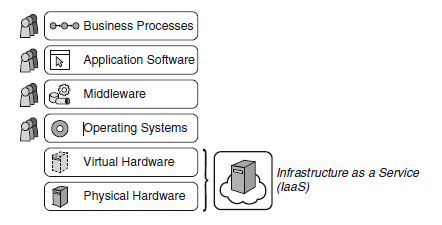
\includegraphics{Gambar/iaas-infrastruktur}
		\caption{Infrastruktur as a Service Stack}
		\label{fig:iaas-infrastruktur}
	\end{figure}
	\item Platform as a Service (PaaS)\\
	merupakan layanan yang menyediakan computing platform. Biasanya sudah terdapat sistem operasi, database, web server dan framework aplikasi agar dapat menjalankan aplikasi yang telah dibuat.
	\begin{figure}[h]
		\centering
			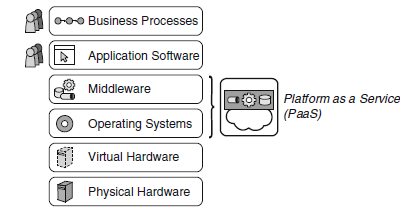
\includegraphics{Gambar/paas-infrastruktur}
		\caption{Infrastruktur as a Service Stack}
		\label{fig:paas-infrastruktur}
	\end{figure}
	\item Software as a Service (SaaS)\\
	merupakan layanan komputasi awan dimana kita bisa langsung menggunakan aplikasi yang telah disediakan.
	\begin{figure}[h]
		\centering
			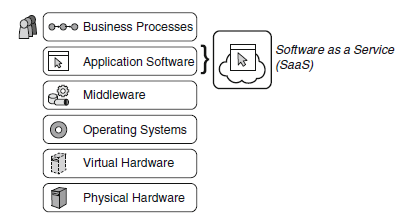
\includegraphics{Gambar/saas-infrastruktur}
		\caption{Infrastruktur as a Service Stack}
		\label{fig:saas-infrastruktur}
	\end{figure}
\end{itemize}

\subsection{Pengenalan \textit{Mobile Cloud Computing}}
\label{subsec:pengenalanmcc}
\hspace{0,5cm} Selama beberapa tahun terakhir perkembangan teknologi informasi dan komunikasi menjadi sangat pesat. Perkembangan teknologi informasi dan komunikasi tersebut mendorong era internet. Karena perkembangan internet, \textit{Cloud Computing} banyak dijadikan topik penelitian dari pada peneliti dan industri. Selanjutnya sifat \textit{Cloud Computing} menguntungkan perangkat dengan komputasi yang terbatas. Karena hal tersebut, perangkat \textit{mobile} diuntungkan karena sebagian komputasi dilakukan \textit{Cloud Computing} dan harga perangkat \textit{mobile} yang relatif murah\cite{mcc}.  

\subsection{Konsep dan Prinsip \textit{Mobile Cloud Computing}}
\label{subsec:konsepmcc}
\hspace{0,5cm} Secara sederhana \textit{Mobile Cloud Computing} mengacu  pada infrastruktur, dimana penyimpanan data dan pemrosesan data terjadi diluar perangkat \textit{mobile}\cite{mcc}. Karena hal tersebut perangkat \textit{mobile} akan mengkonsumsi daya yang lebih sedikit. Infrastruktur \textit{Mobile Cloud Computing} dapat dilihat pada gambar ~\ref{fig:MobileCloudComputing}.

\begin{figure}[h]
	\centering
		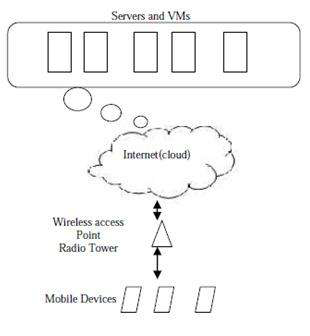
\includegraphics{Gambar/mms_prinsip}
	\caption{\textit{Mobile Cloud Computing}}
	\label{fig:MobileCloudComputing}
\end{figure}
	
\hspace{0,5cm} Arsitektur umum \textit{Mobile Cloud Computing} ditunjukkan pada gambar ~\ref{fig:Arsitekture MobileCloudComputing}\cite{mcc}. Perangkat \textit{mobile} terhubung ke jaringan melalui BTS (misalnya, base station transceiver (BTS), jalur akses, atau satelit) yang membangun dan mengendalikan koneksi dan antarmuka fungsional antara jaringan dan perangkat \textit{mobile}. Permintaan dari ponsel pengguna dan informasi (misalnya, ID, dan lokasi) ditransmisikan ke pusat komputasi yang terhubung ke server . Di sini, operator jaringan mobile dapat memberikan layanan kepada pengguna ponsel sebagai AAA (\textit{Authentication}, Otorisasi, dan Akuntansi) berdasarkan \textit{home agent} (HA) dan data pelanggan yang disimpan dalam database. Setelah itu,
permintaan pelanggan yang dikirim ke awan melalui Internet. Di awan, pengendali awan memproses permintaan untuk memberikan pengguna ponsel dengan layanan \textit{cloud} yang sesuai. Layanan ini dikembangkan dengan konsep utilitas komputasi, virtualisasi, dan layanan arsitektur berorientasi.
	
\begin{figure}[h]
	\centering
		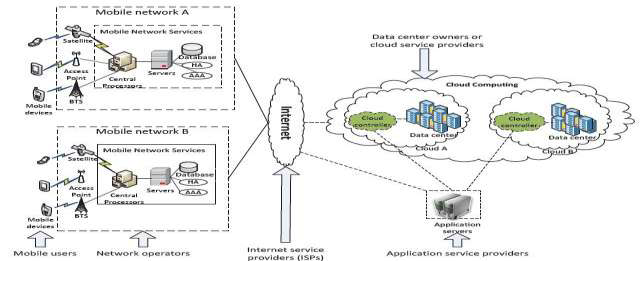
\includegraphics[scale=0.7]{Gambar/mcc_arsitektur}
	\caption{Arsitektur \textit{Mobile Cloud Computing}}
	\label{fig:Arsitekture MobileCloudComputing}
\end{figure}


\section{Android}
\label{sec:android}

Pada sub-bab ini akan dibahas mengenai pengertian dan arsitektur Android.

\subsection{Pengertian Android}
\label{subsec:pengertianandroid}

Android merupakan sistem operasi buatan Google untuk \textit{mobile device}. Saat penelitian ini dilakukan Sistem operasi Android menjadi yang paling populer dan sudah digunakan oleh lebih dari 100 juta pengguna di seluruh dunia\footnote{\url{http://developer.android.com/about/index.html}}. Kesuksesan Android tidak lepas dari basis \textit{open-source} yang memungkinkan pembuatan varian kustom dari Android.
%http://developer.android.com/index.html
%about -> http://developer.android.com/about/index.html

\subsection{Arsitektur Android}
\label{subsec:arsitektur}

Secara umum arsitektur Android dibagi menjadi empat lapisan. Lapisan arsitektur Android dapat dilihat pada Gambar~\ref{fig:arsitektur_android}\footnote{\url{http://elinux.org/Android\_Architecture}}. Berikut ini adalah penjelasan mengenai empat lapisan pada arsitektur Android.

\begin{enumerate}
\item \textit{Applications} merupakan lapisan teratas yang berhubungan dengan pengguna.
\item \textit{Applications Framework} merupakan lapisan yang digunakan oleh para penggembang aplikasi. Pada lapisan ini terdapat \textit{framework} yang dapat digunakan orang para pengembang aplikasi. %Jelasin apa itu framework
\item \textit{Libraries} merupakan kumpulan-kumpulan fungsi yang disediakan oleh Android.
\item \textit{Linux Kernel} merupakan kumpulan-kumpulan fungsi yang berhubungan langsung dengan perangkat keras.
\end{enumerate}

\begin{figure}[h]
\centering
\resizebox{\textwidth}{!}{
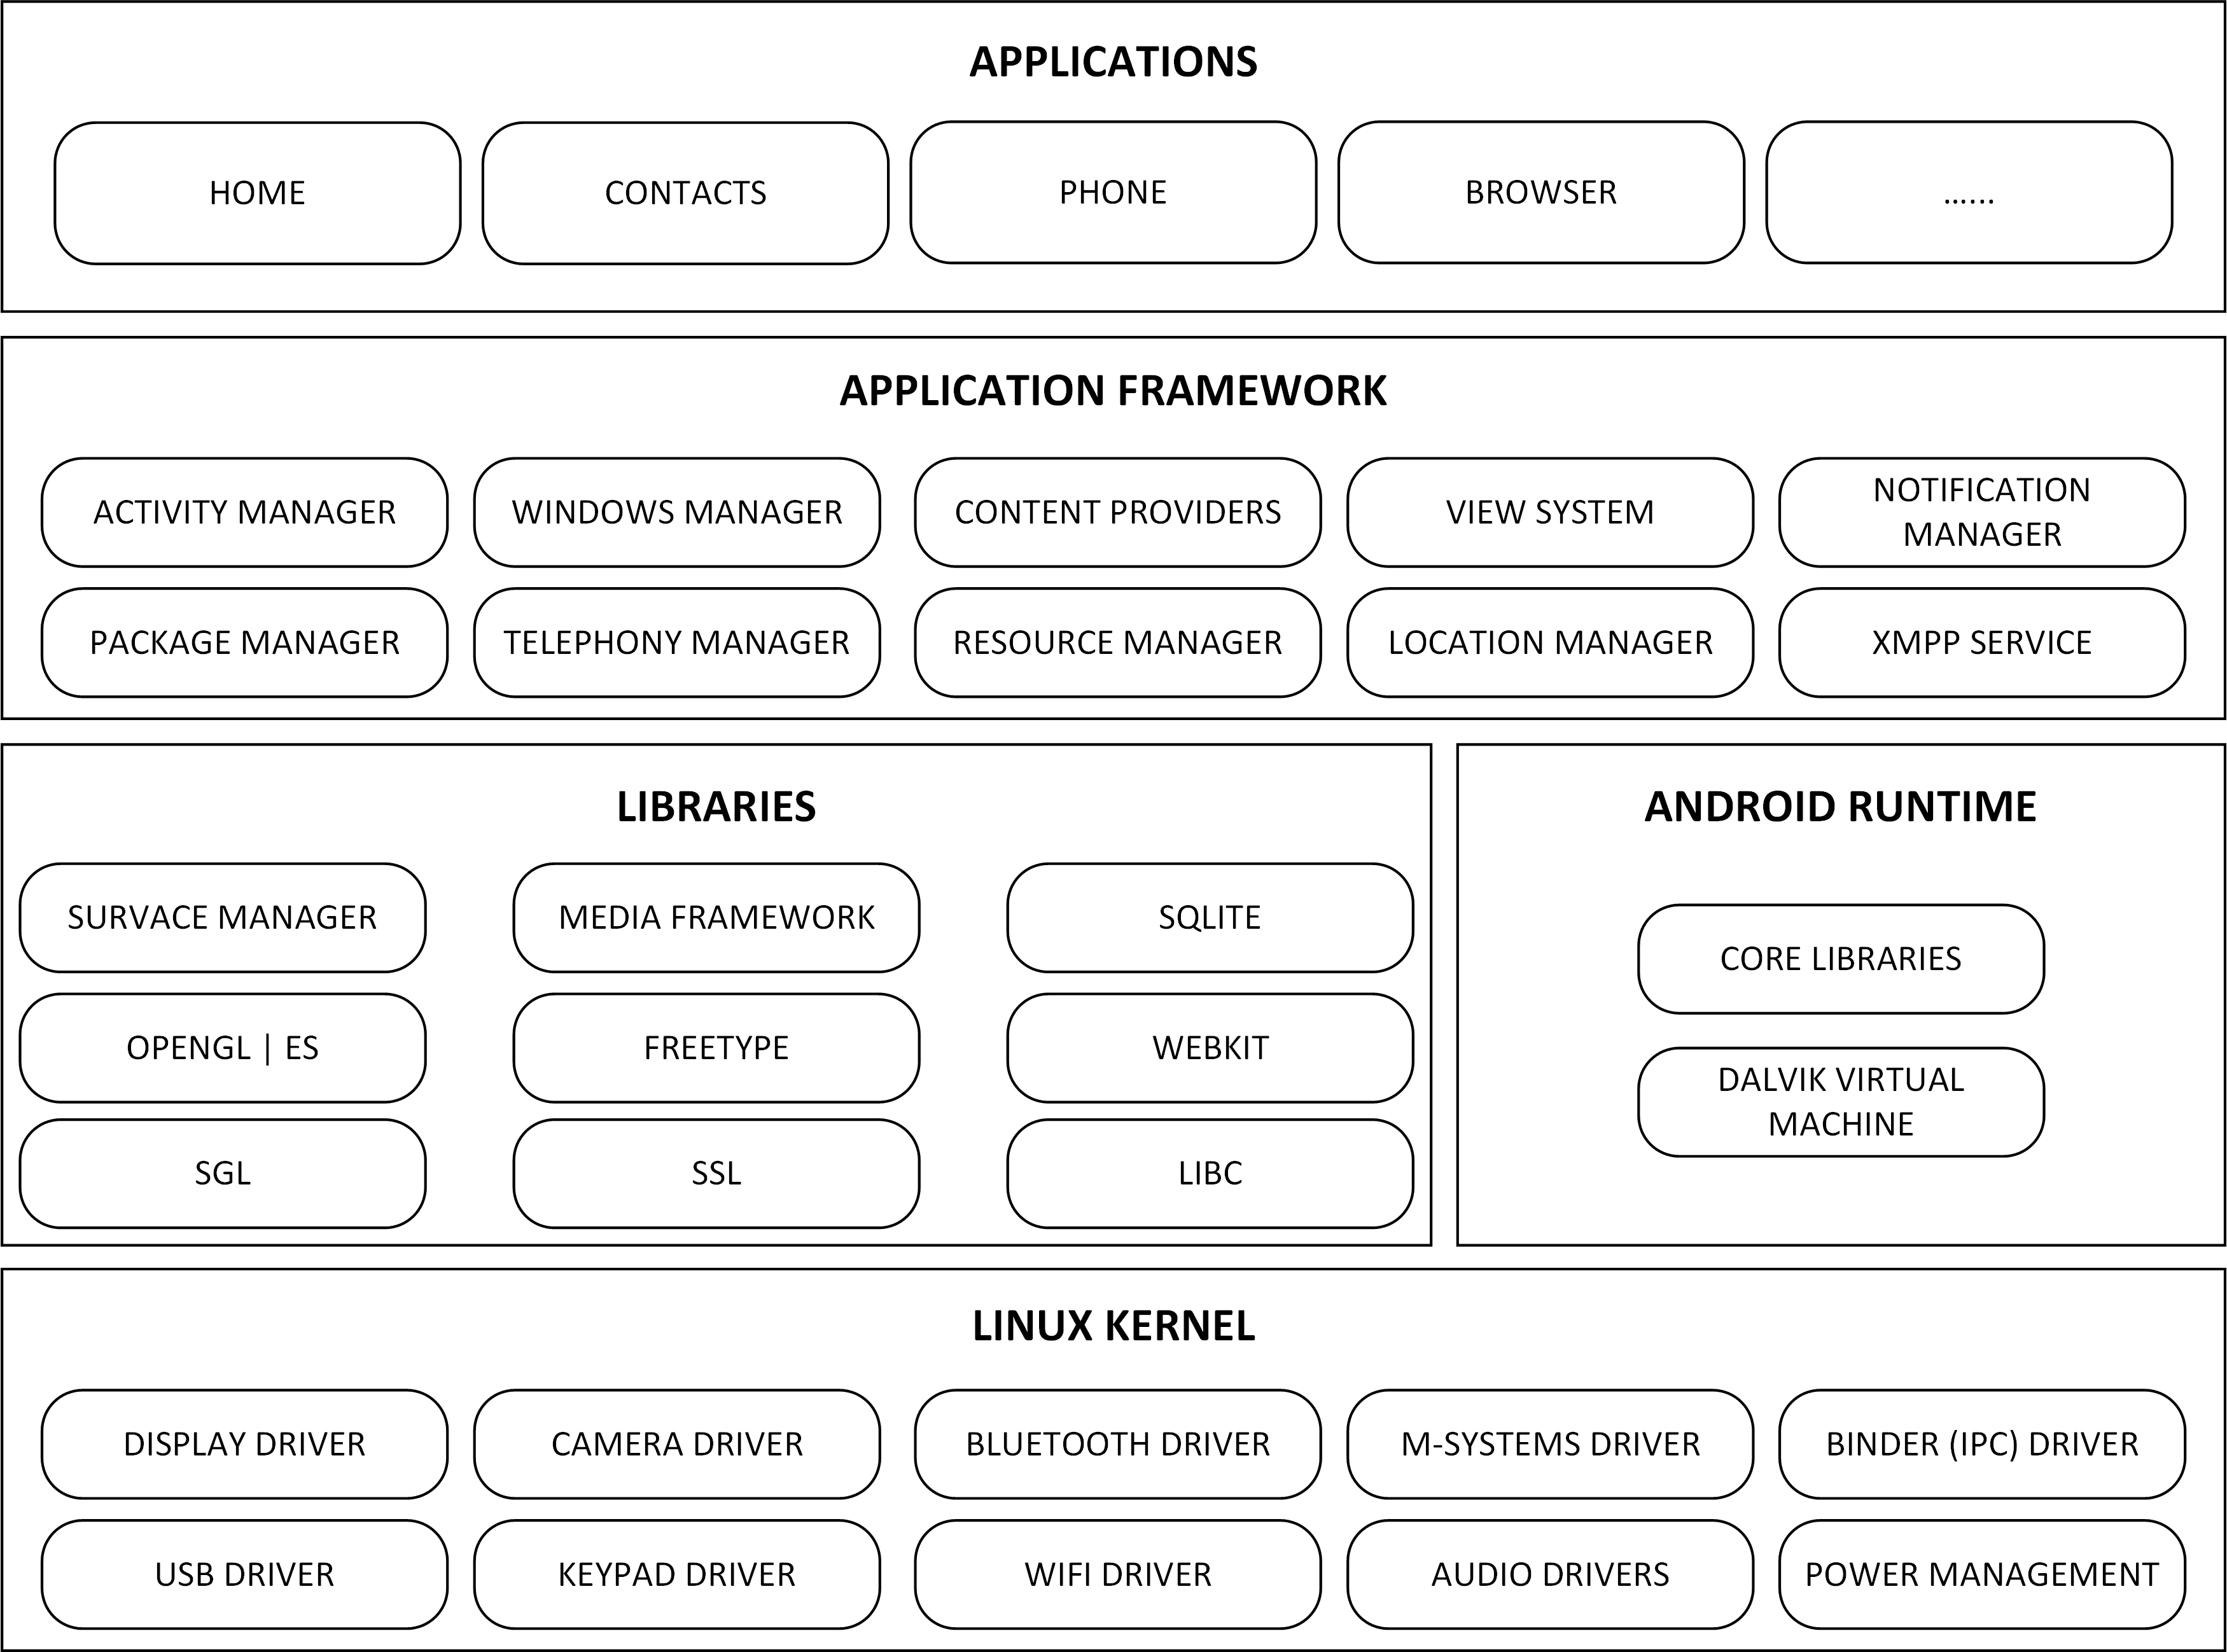
\includegraphics{Gambar/Android-system-architecture}
}
\caption[Arsitektur Android]{Arsitektur Android} 
\label{fig:arsitektur_android}
\end{figure}

\subsection{\textit{Life Cycle}}
\label{subsec:lifecycle}

Aplikasi yang berjalan pada Android memiliki \textit{lifecycle} sesuai dengan rancangan sistem operasi Anrdroid. \textit{Lifecycle} aplikasi pada Android dapat dilihat pada gambar \ref{fig:dasar_lifecycle_android}.

\begin{figure}[h]
\centering
\resizebox{\textwidth}{!}{
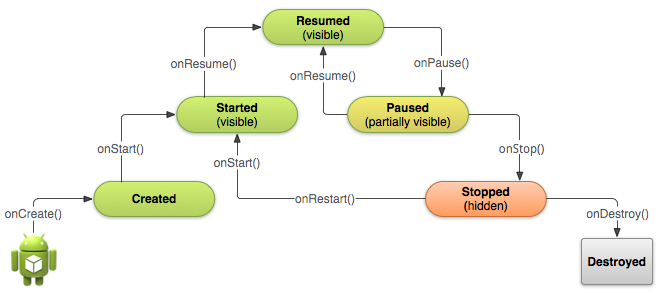
\includegraphics{Gambar/basic-lifecycle}
}
\caption[Dasar \textit{lifecycle} Android]{Dasar \textit{lifecycle} Android} 
\label{fig:dasar_lifecycle_android}
\end{figure}

\section{Phonegap}
\label{sec:phonegap}

\subsection{Pengertian Phonegap}
\label{sec:pengertianphonegap}

Phonegap merupakan suatu \textit{framework} yang digunakan untuk mengembangkan aplikasi pada perangkat mobile. Phonegap memungkinkan aplikasi dibangun di atas Javascript, HTML5, dan CSS3\footnote{Jose Fermoso (April 5, 2009). "PhoneGap Seeks to Bridge the Gap Between Mobile App Platforms"}.

\subsection{Arsitektur Phonegap}
\label{sec:arsitekturphoengap}

Phonegap menggunakan HTML\ref{subsec:html} dan CSS\ref{subsec:css} untuk me-\textit{render} aplikasi dan Javascript\ref{subsec:javascript} digunakan untuk menjalankan logika dari aplikasi yang dibuat. Phonegap membangun API yang dapat digunakan oleh pengembang aplikasi di atas OS \textit{mobile device}. Arsitektur Phonegap dapat dilihat pada Gambar~\ref{fig:arsitektur_phonegap} 

\begin{figure}[h]
\centering
\resizebox{\textwidth}{!}{
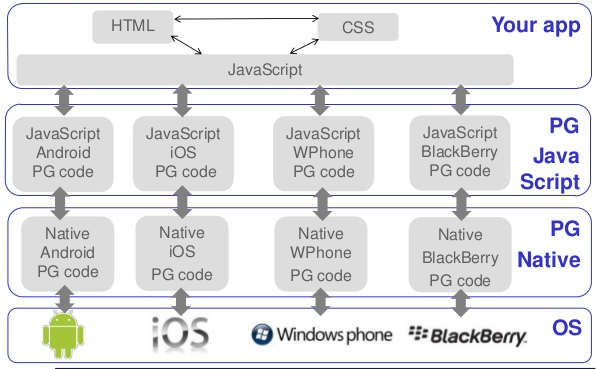
\includegraphics{Gambar/phonegap-architecture}
}
\caption[Arsitektur Phonegap]{Arsitektur Phonegap} 
\label{fig:arsitektur_phonegap}
\end{figure}

Teknologi dasar yang digunakan untuk membangun aplikasi menggunakan Phonegap:
\begin{enumerate}
	\item HTML merupakan suatu bahasa standar yang digunakan untuk membuat halaman situs\footnote{\url{http://www.merriam-webster.com/dictionary/hypertext markup language}}. Contoh penggunaan dapat dilihat pada Gambar~\ref{fig:contoh_html} dan tampilan hasil dapat dilihat pada Gambar~\ref{fig:hasil_contoh_html}
		\begin{figure}[h]
		\centering
		\resizebox{\textwidth}{!}{
		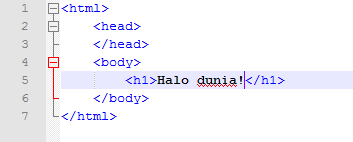
\includegraphics{Gambar/contoh-html}
		}
		\caption[Contoh HTML]{Contoh HTML} 
		\label{fig:contoh_html}
		\end{figure}
		\begin{figure}[h]
		\centering
		\resizebox{\textwidth}{!}{
		
\includegraphics{Gambar/hasil-contoh-html}
		}
		\caption[Hasil contoh HTML]{Hasil contoh HTML} 
		\label{fig:hasil_contoh_html}
		\end{figure}
	\item CSS merupakan suatu bahasa yang digunakan untuk menformat tampilan suatu dokumen. Contoh penggunaan dapat dilihat pada Gambar~\ref{fig:contoh_html_css} dan tampilan hasil dapat dilihat pada Gambar~\ref{fig:hasil_contoh_html_css}
		\begin{figure}[h]
		\centering
		\resizebox{\textwidth}{!}{
		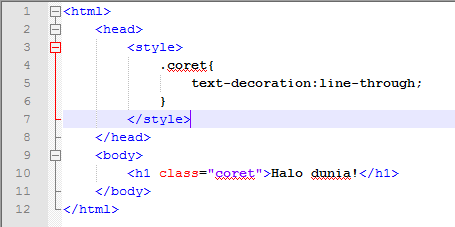
\includegraphics{Gambar/contoh-html-css}
		}
		\caption[Contoh CSS pada dokumen HTML]{Contoh CSS pada dokumen HTML} 
		\label{fig:contoh_html_css}
		\end{figure}
		\begin{figure}[h]
		\centering
		\resizebox{\textwidth}{!}{
		
\includegraphics{Gambar/hasil-contoh-html-css}
		}
		\caption[Hasil contoh CSS pada dokumen HTML]{Hasil contoh CSS pada dokumen HTML} 
		\label{fig:hasil_contoh_html_css}
		\end{figure}
	\item Javascript merupakan bahasa pemograman yang pada umumnya digunakan pada \textit{web browser}. Contoh penggunaan dapat dilihat pada Gambar~\ref{fig:contoh_js} dan tampilan hasil dapat dilihat pada Gambar~\ref{fig:hasil_js}
		\begin{figure}[h]
		\centering
		\resizebox{\textwidth}{!}{
		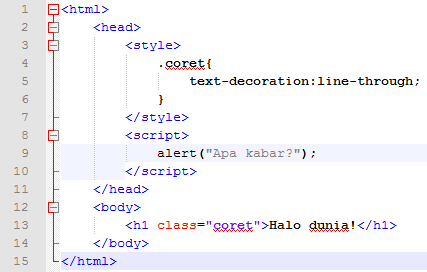
\includegraphics{Gambar/contoh-js}
		}
		\caption[Contoh Javascript pada dokumen HTML]{Contoh Javascript pada dokumen HTML} 
		\label{fig:contoh_js}
		\end{figure}
		\begin{figure}[h]
		\centering
		\resizebox{\textwidth}{!}{
		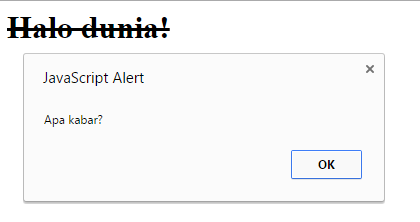
\includegraphics{Gambar/hasil-js}
		}
		\caption[Hasil contoh Javascript]{Hasil contoh Javascript} 
		\label{fig:hasil_js}
		\end{figure}
\end{enumerate}

Selain tiga teknologi dasar yang digunakan untuk membangunan aplikasi di Phonegap, terdapat teknologi lain yaitu:
\begin{enumerate}
	\item Jquery merupakan suatu \textit{libary} javascript yang dibangun untuk memanipulasi dokumen HTML.
	\item AngularJS merupakan suatu \textit{framework} yang ditulis diatas javascript yang digunakan untuk memanipulasi dokumen HTML.
	\item Onsen UI\footnote{\url{http://onsen.io/}} merupakan suatu \textit{framework} Javascript  dan CSS untuk membangun aplikasi HTML atau Phonegap.
\end{enumerate}

\section{CakePHP}

CakePHP merupakan sebuah \textit{framework} yang digunakan untuk membangun suatu aplikasi \textit{web}. Cakephp mengikuti konsep MVC yang ditulis diatas PHP.

\section{Hadoop dan ekosistem}
\label{sec:hadoopdanekosistem}

Hadoop merupakan sebuah \textit{platform} yang menyediakan pemyimpanan data terdistribusi dan kemampuan komputasi. Kemampuan komputasi pada Hadoop merupakan \textit{distributed master-slave architeture} yang terdiri dari Hadoop Distributed File System (HDFS)\ref{subsec:hdfs} untuk penyimpanan data dan MapReduce \ref{subsec:mapreduce}. Arsitektur Hadoop dapat dilihat pada Gambar \ref{fig:arsitektur_hadoop}\cite{holmes2012hadoop}.

\begin{figure}
\centering
\resizebox{\textwidth}{!}{
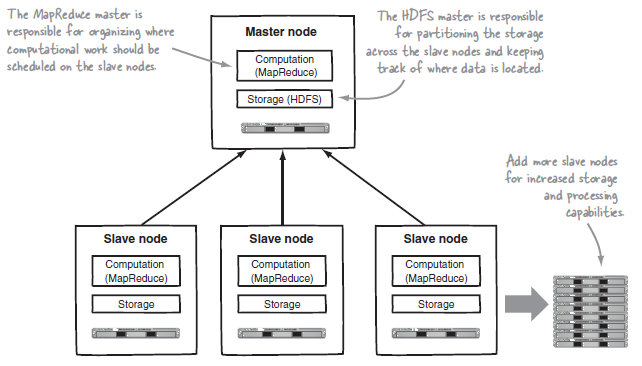
\includegraphics{Gambar/high-level-hadoop-architecture}
}
\caption[Arsitektur Hadoop]{Arsitektur Hadoop} 
\label{fig:arsitektur_hadoop}
\end{figure}

Beberapa ekosistem yang ada pada \textit{Hadoop} berupa:

\begin{enumerate}
	\item HDFS adalah komponen penyimpanan data dari Hadoop yang merupakan sistem penyimpanan data terdistribusi. Arsitektur HDFS dapat dilihat pada Gambar \ref{fig:arsitektur_hdfs}
	\item MapReduce merupakan \textit{batch-based}, komputasi terdistribusi \textit{framework} yang memungkinkan komputasi paralel terhadap data yang cukup besar. MapReduce menyederhanakan pemrosesan paralel oleh abstraksi kerja yang komplek. Dengan abstraksi ini, MapReduce memungkinkan \textit{programmer} untuk berfokus pada kebutuhan bisnis dibandingkan memikirkan sistem distribusinya.
	\item HBase merupakan \textit{real-time, column-oriented} basis data yang dapat diintergrasi kedalam HDFS melalu MapReduce.
\end{enumerate}

\begin{figure}
\centering
\resizebox{\textwidth}{!}{
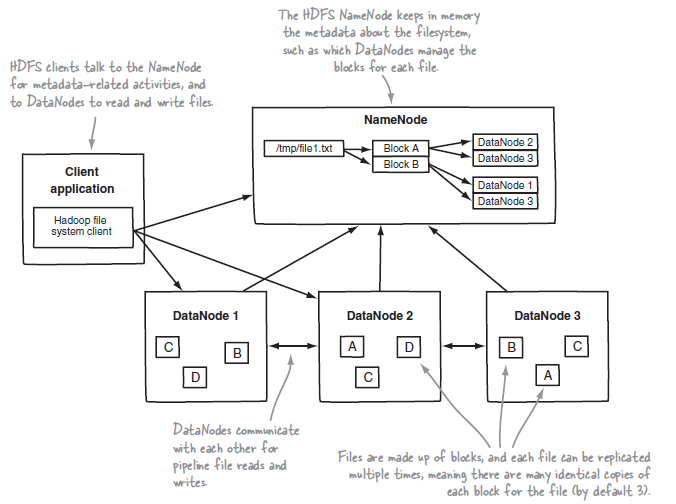
\includegraphics{Gambar/arsitektur-hdfs}
}
\caption[Arsitektur HDFS]{Arsitektur HDFS} 
\label{fig:arsitektur_hdfs}
\end{figure}

Selain ekosistem \textit{Hadoop} sendiri, terdapat beberapa teknologi pendukungnya, berupa:

\begin{enumerate}
	\item Trafodion merupakan \textit{open source project} yang disponsor oleh HP. Trafodion juga diinkubasi di HP Labs dan HP-IT yang digunakan untuk mengembangkan SQL-on-Hadoop berskala \textit{enterprise} terhadap data yang besar\footnote{\url{https://wiki.trafodion.org/wiki/index.php/Main\_Page}}. Trafodion digunakan untuk membuat \textit{Hbase} menjadi basis data yang dapat di-\textit{query} menggunakan bahasa SQL.
	\item SQL(\textit{Structured Query Language}) merupakan suatu bahasa pemograman yang didisain untuk mengelolah data yang terdapat pada \textit{relational database management system}(RDBMS).
\end{enumerate}

\section{Webservice}
\label{sec:webservice}

Webservice merupakan suatu sistem yang menyediakan fungsi-fungsi dari suatu perangkat lunak diatas internet melalui \textit{web}.

Adapun beberapa teknologi yang terkait dengan webservice:
\begin{enumerate}
	\item \textit{Representational State Transfer}(REST) merupakan gaya arsitektur suatu perangkat lunak yang terdiri dari pedoman dan praktek terbaik untuk membuat suatu \textit{webservice} yang \textit{scalable}\footnote{Fielding, R. T.; Taylor, R. N. (2000). "Principled design of the modern Web architecture". pp. 407\-416. doi:10.1145/337180.337228}
	\item \textit{Hypertext Transfer Protocol}(HTTP) merupakan suatu protokol aplikasi untuk sistem informasi yang terdistribusi, kolaborasi dan hipermedia.Pada HTTP terdapat beberapa protokol, yakni:
	\begin{itemize}
		\item \textit{OPTIONS}
		\item \textit{GET}
		\item \textit{HEAD}
		\item \textit{POST}
		\item \textit{PUT}
		\item \textit{DELETE}
		\item \textit{TRACE}
		\item \textit{CONNECT}
	\end{itemize}
	\item \textit{Uniform Resource Identifier}(URI) merupakan urutan kompak karakter yang mengidentifikasikan sumber daya abstrak dan fisik\cite{rfc3986}.
	\item \textit{Javascript Object Notation}(JSON) merupakan suatu teks format yang digunakan untuk serialisasi struktur data\cite{rfc7159}.
\end{enumerate}

\section{Google Open Authentication (OAuth)}
\label{sec:googleopenauthentication}

Pada sub-bab ini akan dibahas mengenai OAuth dan Google Oauth.

\subsection{Open Authentication (OAuth)}
\label{subsec:oauth}

\hspace{0,5cm}OAuth merupakan standar terbuka untuk autentikasi. Oauth menyediakan akses yang aman kepada klien untuk mengakses \textit{server}. Hal ini menjadikan \textit{server} dapat diakses oleh \textit{third-party}. Desain OAuth diatas HTTP. Prinsip OAuth pada dasarnya menyediakan akses token kepada klien/pengguna akhir sehingga dapat digunakan untuk bertransaksi dengan \textit{server}\cite{rfc6749}.

\subsection{Google \textit{OAuth}}
\label{subsec:googleip}

\hspace{0,5cm}Google OAuth merupakan protokol OAuth yang digunakan oleh google untuk memberikan akses kepada \textit{third-party} untuk mengakses API mereka. Skema untuk mengakses Google OAuth dapat dilihat pada Gambar~\ref{fig:google_oauth}.

\begin{figure}[h]
\centering
\resizebox{\textwidth}{!}{
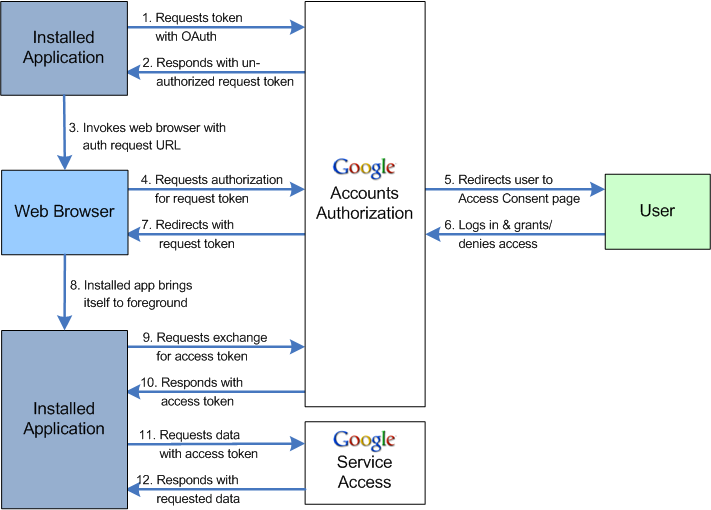
\includegraphics{Gambar/google-oauth}
}
\caption[Google OAuth]{Google OAuth} 
\label{fig:google_oauth}
\end{figure}

\subsection{Google \textit{Identity Platform}}
\label{subsec:googleidentityplatform}
\hspace{0,5cm} Merupakan layanan dari Google yang memberikan kemudahan dan keamanan  untuk masuk ke situs dan aplikasi dengan mudah. Untuk memanfaatkan layanan dibutuhkan pemanfaatan API di situs maupun aplikasi. Solusi layanan yang dapat digunakan untuk Android, iOS, dan situs adalah Google Sign-In\cite{android}. Berikut kegunaan dari Google Sign-In.
\begin{itemize}
	\item Mendapatkan pengguna untuk mengakses aplikasi dengan cepat dan aman dengan pengembangan yang sedikit. 
	\item Pengguna cukup \textit{sign-in} sekali dan di \textit{authenticated} di semua perangkat mereka.
	\item Layanan Google yang terintegrasi
	\item Memungkinkan instalasi dari aplikasi Android ketika pengguna masuk ke situs
\end{itemize}
   
%API = https://developers.google.com/identity/sign-in/web/sign-in}{}
\ifdefstring{\vbabc}{1}{\chapter{Analisis}
\label{chap:analisis}

\section{Deskripsi Masalah}
\label{sec:deskripsimasalah}

\hspace{0,5cm}Untuk mengolah keuangan sebuah rumah tangga tidaklah mudah. Rumah tangga memiliki beberapa anggota yang terdiri dari kepala, pengurus dan anggota(anak) rumah tangga. Tentunya pengololahan rumah tangga dilakukan oleh kepala rumah tangga atas semua transaksi keuangan yang dilakukan oleh anggota rumah tangga. Untuk melaporkan semua transaksi yang dilakukan oleh anggota rumah tangga kepada kepala rumah tangga terkadang terhalang oleh komunikasi apalagi jika kepala dan anggota rumah tangga tinggal ditempat yang berbeda.

Dari masalah tersebut, akan dibuat suatu aplikasi yang dapat membantu suatu rumah tangga dalam pengelolaan keuangan mereka. Aplikasi ini dapat digunakan oleh setiap anggota rumah tangga untuk mencatat semua transaksi yang mereka lakukan baik pengeluaran maupun pendapatan. Aplikasi ini juga dapat menampilkan laporan sesuai dengan transaksi yang telah tercatat.

Aplikasi ini sendiri terbagi menjadi dua bagian yaitu aplikasi \textit{end-user} yang digunakan langsung oleh para anggota rumah tangga dan aplikasi yang digunakan oleh admin untuk mengelolah data-data aplikasi.

Data-data yang tercatat tentunya akan disimpan kedalam sebuah basis data sehingga aplikasi ini sendiri akan berkomunikasi dengan \textit{server} yang berfungsi sebagai penyimpanan dan pengolahan data yang dibangun diatas \textit{framework} Hadoop. Untuk komunkasi aplikasi dan \textit{server} akan menggunakan HTTP dimana aplikasi akan mengakses \textit{webservice} yang telah disediakan oleh \textit{server}.

\section{\textit{Mobile Cloud Computing Model} untuk Pembukuan Rumah Tangga}

Pada permodelan dipenelitian ini menggunakan \textit{Mobile Cloud Computing Model} dimana aplikasi akan berkomunikasi dengan \textit{server} melalui \text{webservice} diatas HTTP. \textit{Webservice} akan gerbang bagi aplikasi untuk memanipulasi data. Untuk bagian \textit{back-end}, \textit{webservice} akan ditulis di atas PHP dan menggunakan Trafodion untuk memanipulasi data diatas Hadoop. Gambaran model dapat dilihat pada Gambar~\ref{fig:prt_architecture}

\begin{figure}[h]
\centering
\resizebox{\textwidth}{!}{
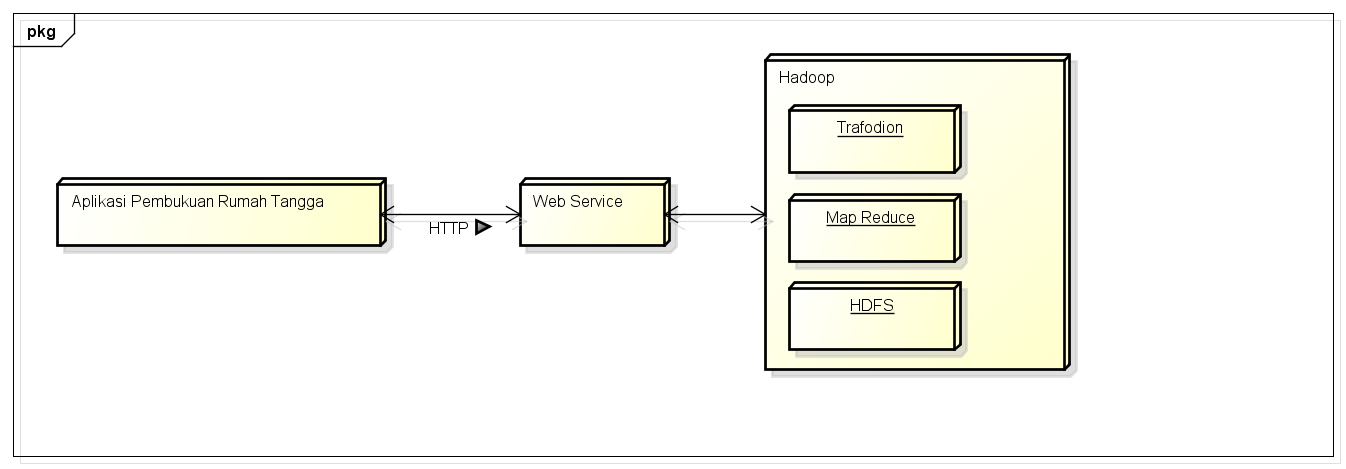
\includegraphics{Gambar/prt-architecture}
}
\caption[Permodelan Pembukuan Rumah Tangga]{Permodelan Pembukuan Rumah Tangga} 
\label{fig:prt_architecture}
\end{figure}

\section{Analisis Kebutuhan Perangkat Lunak}

\hspace{0,5cm}Pada sub-bab ini akan dibahas mengenai analisis terhadap perangkat lunak yang akan dikembangkan.

\subsection{Analisis Aplikasi \textit{Mobile Device}}

Pada aplikasi \textit{mobile device} akan ditujukan kepada pengguna rumah tangga untuk mengelolah transaksi yang mereka lakukan. Aplikasi ini memiliki beberapa fitur utama dan tiga peran.

\hspace{0,5cm}Peran yang ada pada aplikasi ini yakni:
\begin{enumerate}
	\item Kepala rumah tangga
	\item	Pengurus rumah tangga
	\item Anggota rumah tangga
\end{enumerate}

Fitur-fitur yang ada, yakni:
\begin{enumerate}
	\item Pendaftaran diri, pendaftaran dilakukan untuk mendapatkan hak akses kedalam sistem aplikasi dan pendaftaran mendapat peran sebagai kepala rumah tangga
	\item Pengisian profil rumah tangga, pengisian profil dilakukan oleh kepala rumah tangga setelah mendaftarkan diri dan disetujui oleh admin
	\item	Mendaftarkan pengurus dan anggota rumah tangga, kepala rumah tangga dapat menambahkan dan mengurungai pengurus dan anggota rumah tangga yang berelasi terhadapnya
	\item Mencatat transaksi, semua peran mendapat hak akses untuk fitur ini dimana fitur ini untuk mencatat transaksi keuangan masing-masing.
	\item Alokasi keuangan, fitur ini berupa transfer dana antar anggota rumah tangga, baik dari kepala ke anggota dan sebaliknya, fitur ini hanya dimiliki oleh kepala dan pengurus rumah tangga.
	\item Menambah kategori transaksi, fitur ini hanya dimiliki oleh kepala rumah tangga yang bertujuan untuk menambah kategori transaksi.
	\item Melihat laporan keuangan, fitur ini hanya dapat diakses oleh kepala dan penguru rumah tangga.
	\item Melihat transaksi, fitur ini dapat diakses oleh semua peran rumah tangga.
\end{enumerate}

Penulis akan mengembangkan aplikasi \textit{mobile device} menggunakan Phonegap yang ditulis diatas \textit{webview} tetapi aplikasi ini tidak akan berjalan diatas \textit{web browser} karena Phonegap yang akan meng-\textit{compile} aplikasi ini sehingga akan menjadi suatu aplikasi Android.Untuk tampilan dasar pada aplikasi, penulis menggunakan \textit{framework} Onsen-UI yang dibangun diatas AngularJS. Penulis memilih \textit{framework} ini karena merupakan \textit{single page web} yang cocok untuk membuat aplikasi yang hendak dibangun penulis. Selain menggunakan AngularJS, penulis juga mengguna Jquery untuk memanipulasi data pada aplikasi.


\subsection{Analisis Aplikasi \textit{Website}}

\hspace{0,5cm}Aplikasi \textit{website} ini dibuat hanya untuk admin sehingga dapat mengatur data-data yang ada pada aplikasi.

Fitur-fitur yang ada yakni:
\begin{enumerate}
	\item Pengolahan anggota
				Admin dapat menyetujui atau menolak pendaftaran dari pengguna
	\item	Pengolahan kategori transaksi
				Admin dapat mengurangi atau menambah kategori transaksi
	\item Pelaporan
				Admin dapat membuat laporan secara keseluruhan
\end{enumerate}

Penulis akan mengembangkan aplikasi \textit{website} menggunakan \textit{framework} CakePHP yang ditulis diatas PHP. CakePHP mengikuti disain MVC yang memudahkan untuk membuat suatu aplikasi \textit{website}.

Pada aplikasi ini, terdapat beberapa model berupa:
\begin{itemize}
	\item Anggota yang merepresentasikan anggota pengguna aplikasi \textit{mobile device.}
	\item Kategori yang merepresentasikan kategori-kategori transaksi yang ada.
	\item Rumah Tangga yang merepresentasikan sebuah rumah tangga
	\item Transaksi yang merepresentasikan transaksi yang dilakukan oleh anggota.
	\item Account yang merepresentasikan akun pengguna aplikasi \textit{website}.
	\item Module yang merepresentasikan menu yang ada pada aplikasi \textit{website}.
	\item ModuleContent yang merepresentasikan sub-sub menu yang ada pada aplikasi \textit{website}.
	\item User yang merepresentasikan data login untuk akun pengguna aplikasi \textit{website}.
	\item UserGroup yang merepresentasikan grup akun.
	\item Role yang merepresentasikan hak akses setiap UserGroup.
\end{itemize}

\subsection{Analisis \textit{Webservice}}

\hspace{0,5cm}Aplikasi \textit{mobile device} membutuhkan fungsi-fungsi untuk memanipulasi data. Fungsi-fungsi ini dapat dibangun pada aplikasi \textit{website} dan biasanya disebut dengan \textit{webservice}. Penulis akan membuat webservice yang berfungsi menyediakan layanan untuk aplikasi \textit{mobile device}. Penulis akan membangun webservice diatas PHP, mengikuti disain REST dan menggunakan JSON sebagai respon format data.

Adapun beberapa layanan yang akan dibuat berupa:
\begin{itemize}
	\item Mencatat transaksi.
	\item Menambah dan mengurangi kategori transaksi.
	\item Menyiapkan data laporan.
	\item Melihat anggota rumah tangga.
\end{itemize}

\subsection{\textit{Use Case}}

\hspace{0,5cm}Proses yang akan dilalui dalam bisnis ini berupa:
\begin{enumerate}
	\item Administrator menentukan katagori transaksi yang dapat dipakai oleh semua rumah tangga.
	\item Kepala rumah tangga mendaftarkan diri ke sistem.
	\item Administrator memverifikasi dan menyetujui pendaftaran Kepala rumah tangga.
	\item Kepala rumah tangga yang sudah disetujui pendaftarannya, melengkapi data profil rumah tangganya.
	\item Kepala rumah tangga mendaftarkan pengurus dan anggota rumah tangganya.
	\item Kepala rumah tangga dapat menambahkan atau mengurangi katagori transaksi keuangan yang dapat digunakan dalam rumah tangganya.  
	\item Kepala rumah tangga dapat mengalokasikan katagori transaksi keuangan di dalam rumah tangganya kepada pengurus dan anggota rumah tangga.
	\item Kepala atau pengurus rumah tangga dapat mentransfer uang dari akun induk ke akun anggota rumah tangga.
	\item Kepala atau pengurus rumah tangga dapat memonitor semua transaksi rumah tangganya melalui laporan rumah tangganya.
	\item Semua anggota rumah tangga (termasuk Kepala dan Pengurus) dapat melakukan transaksi keuangan sesuai dengan katagori transaksi keuangan yang telah dialokasikan kepadanya.
\end{enumerate}

\hspace{0,5cm}Diagram \textit{use case} oleh pengguna aplikasi dapat dilihat pada Gambar~\ref{fig:diagram_use_case_mobile}

\begin{figure}[h]
\centering
\resizebox{\textwidth}{!}{
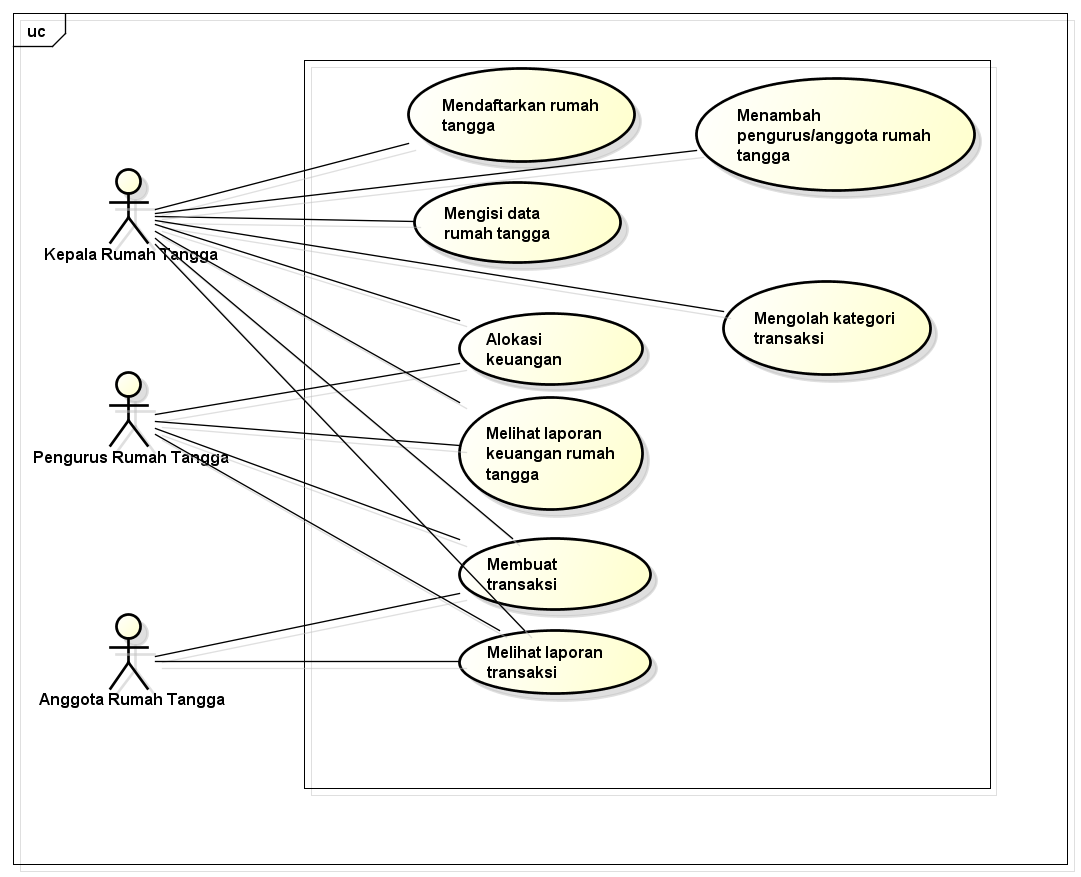
\includegraphics[scale=0.02]{Gambar/use-case-mobile}
}
\caption[Diagram \textit{Use Case Mobile Device}]{Diagram \textit{Use Case Mobile Device}} 
\label{fig:diagram_use_case_mobile}
\end{figure}

Diagram \textit{use case website} yang digunakan admin dapat dilihat pada Gambar~\ref{fig:diagram_use_case_website}

\begin{figure}[h!]
\centering
\resizebox{\textwidth}{!}{
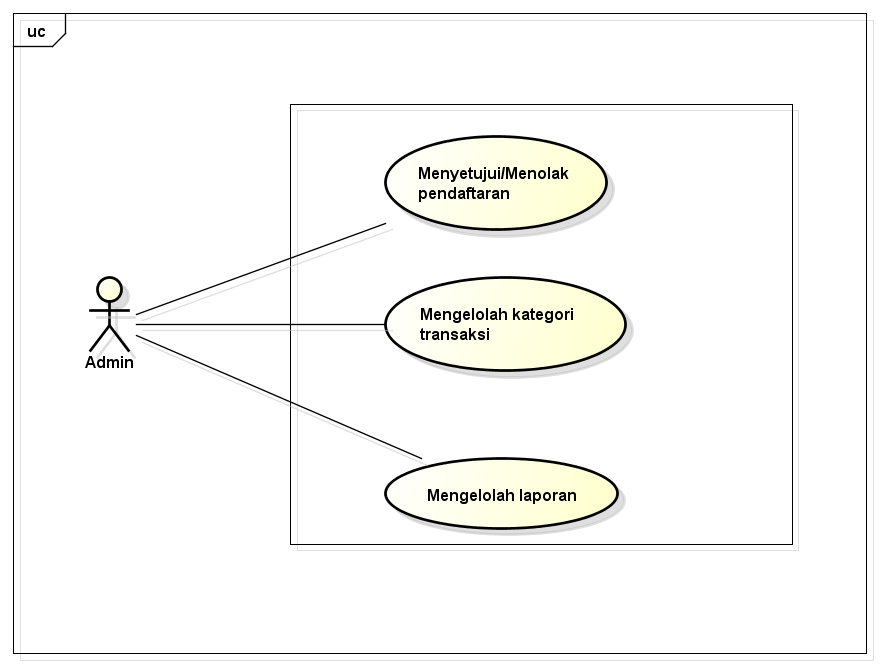
\includegraphics[scale=0.02]{Gambar/use-case-web}
}
\caption[Diagram \textit{Use Case Mobile Website}]{Diagram \textit{Use Case Mobile Website}} 
\label{fig:diagram_use_case_website}
\end{figure}}{}
\ifdefstring{\vbabd}{1}{\chapter{Disain}
\label{chap:disain}

\section{Disain Antarmuka}
\label{sec:disainantarmuka}

\hspace{0,5cm}Pada sub-bab ini akan dibahas mengenai disain antar muka aplikasi \textit{mobile} dan \textit{website}.

\subsection{Disain Aplikasi \textit{Mobile}}
\label{subsec:disainaplikasimobile}

\hspace{0,5cm}Pada aplikasi \textit{mobile} terdapat beberapa halaman utama pendukung fitur, yakni:
\begin{enumerate}
	\item Halaman \textit{login}
	\item	Halaman pendaftaran
	\item Halaman pengisian profil rumah tangga
	\item Halaman \textit{dashboard}
	\item Halaman penambahan anggota
	\item Halaman anggota keluarga
	\item Halaman pengolahan kategori transaksi
	\item Halaman penambahan kategori
	\item Halaman transfer
	\item Halaman penambahan pemasukan
	\item Halaman penambahan pengeluaran
	\item Halaman pemilihan laporan
	\item Halaman laporan
\end{enumerate}

\begin{figure}
\centering
\resizebox{\textwidth}{!}{
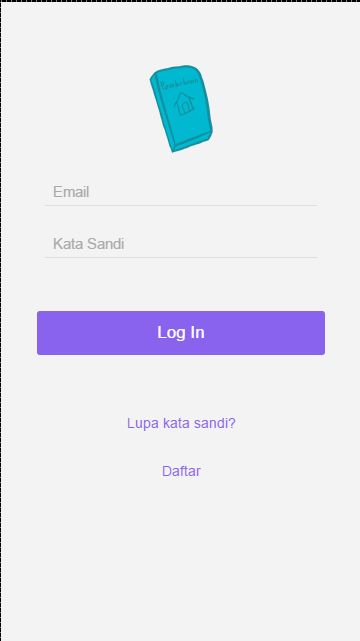
\includegraphics[scale=0.01]{Gambar/design-app/login}
}
\caption[Tampilan \textit{login}]{Tampilan \textit{login}} 
\label{fig:design_app_login}
\end{figure}

\begin{figure}
\centering
\resizebox{\textwidth}{!}{
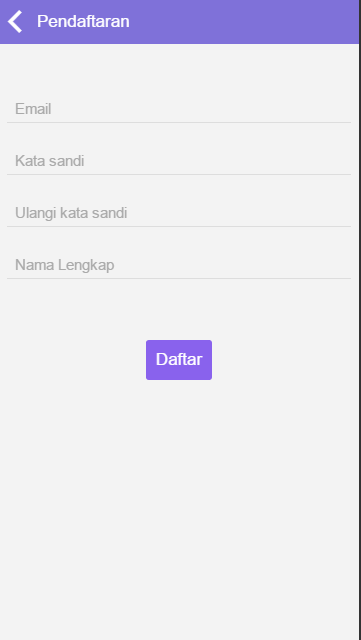
\includegraphics[scale=0.01]{Gambar/design-app/register}
}
\caption[Tampilan pendaftaran]{Tampilan pendaftaran} 
\label{fig:design_app_pendaftaran}
\end{figure}

\begin{figure}
\centering
\resizebox{\textwidth}{!}{
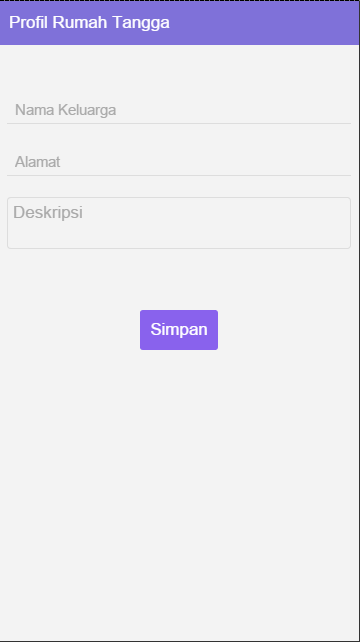
\includegraphics[scale=0.01]{Gambar/design-app/profil_awal}
}
\caption[Tampilan pengisian profil rumah tangga]{Tampilan pengisian profil rumah tangga} 
\label{fig:design_app_profil awal}
\end{figure}

\begin{figure}
\centering
\resizebox{\textwidth}{!}{
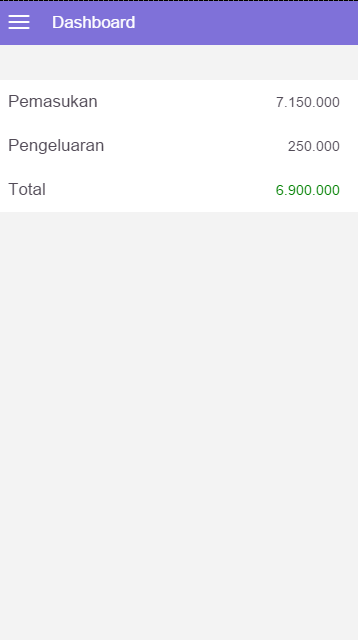
\includegraphics[scale=0.01]{Gambar/design-app/dashboard}
}
\caption[Tampilan \textit{dashboard}]{Tampilan \textit{dashboard}} 
\label{fig:design_app_dashboard}
\end{figure}

\begin{figure}
\centering
\resizebox{\textwidth}{!}{
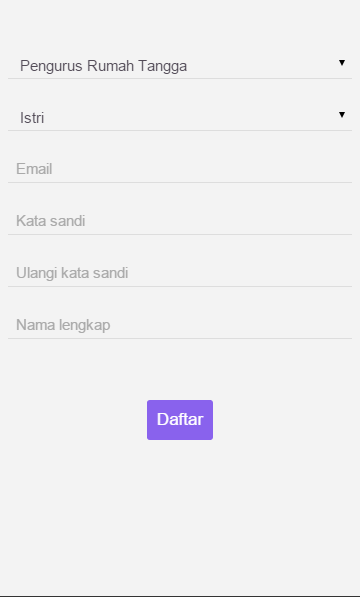
\includegraphics[scale=0.01]{Gambar/design-app/penambahan_anggota}
}
\caption[Tampilan penambahan anggota]{Tampilan penambahan anggota} 
\label{fig:design_app_penambahan_anggota}
\end{figure}

\begin{figure}
\centering
\resizebox{\textwidth}{!}{
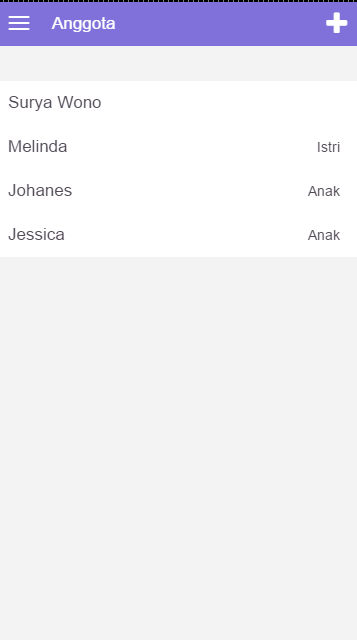
\includegraphics[scale=0.01]{Gambar/design-app/anggota_keluarga}
}
\caption[Tampilan anggota keluarga]{Tampilan anggota keluarga} 
\label{fig:design_app_anggota_keluarga}
\end{figure}

\begin{figure}
\centering
\resizebox{\textwidth}{!}{
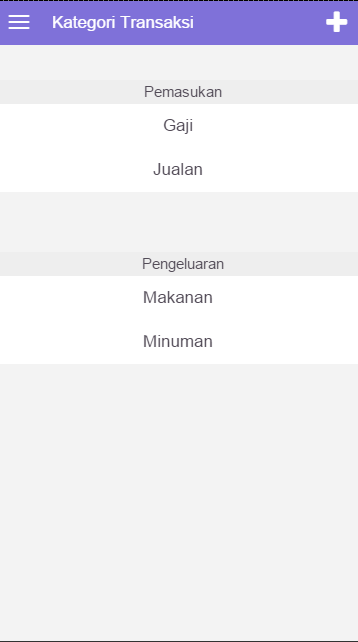
\includegraphics[scale=0.01]{Gambar/design-app/kategori_transaksi}
}
\caption[Tampilan pengolahan kategori transaksi]{Tampilan pengolahan kategori transaksi} 
\label{fig:design_app_kategori_transaksi}
\end{figure}

\begin{figure}
\centering
\resizebox{\textwidth}{!}{

\includegraphics[scale=0.01]{Gambar/design-app/penambahan_kategori}
}
\caption[Tampilan penambahan kategori]{Tampilan penambahan kategori} 
\label{fig:design_app_penambahan_kategori}
\end{figure}

\begin{figure}
\centering
\resizebox{\textwidth}{!}{
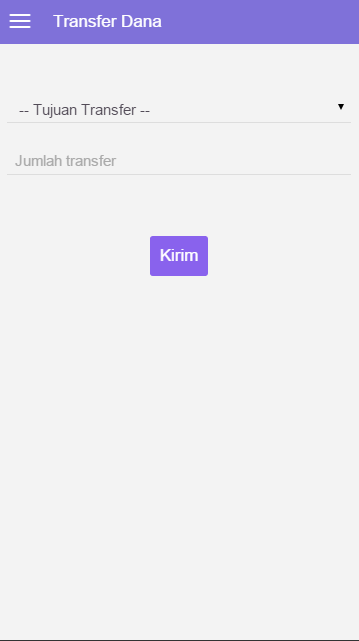
\includegraphics[scale=0.01]{Gambar/design-app/transfer}
}
\caption[Tampilan transfer]{Tampilan transfer} 
\label{fig:design_app_transfer}
\end{figure}

\begin{figure}
\centering
\resizebox{\textwidth}{!}{
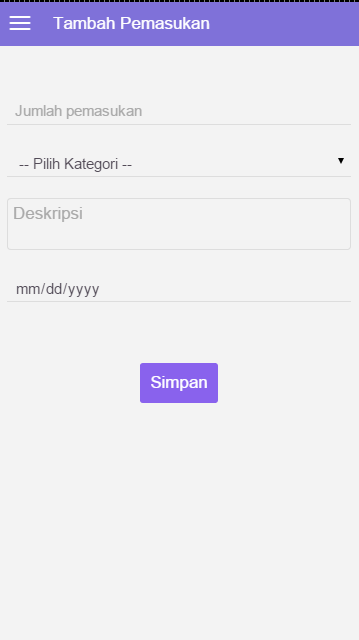
\includegraphics[scale=0.01]{Gambar/design-app/penambahan_pemasukan}
}
\caption[Tampilan penambahan pemasukan]{Tampilan penambahan pemasukan} 
\label{fig:design_app_penambahan_pemasukan}
\end{figure}

\begin{figure}
\centering
\resizebox{\textwidth}{!}{
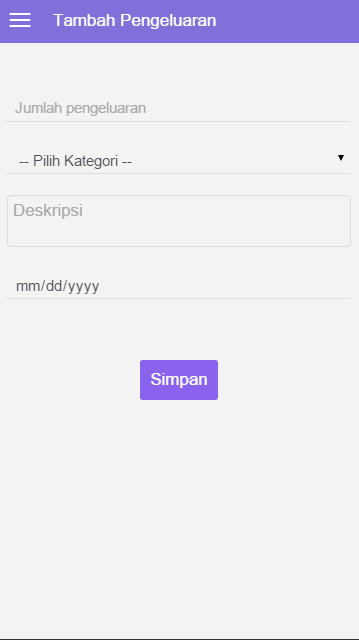
\includegraphics[scale=0.01]{Gambar/design-app/penambahan_pengeluaran}
}
\caption[Tampilan penambahan pengeluaran]{Tampilan penambahan pengeluaran} 
\label{fig:design_app_penambahan_pengeluaran}
\end{figure}

\begin{figure}
\centering
\resizebox{\textwidth}{!}{
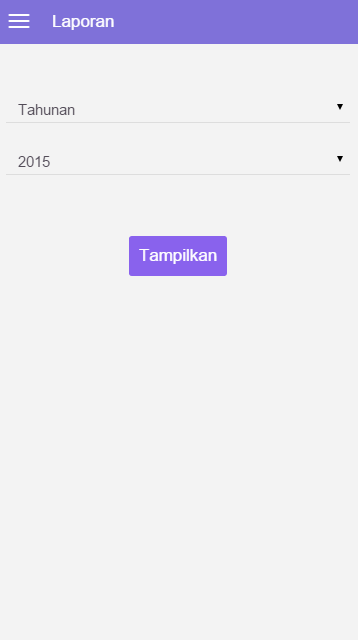
\includegraphics[scale=0.01]{Gambar/design-app/pemilihan_laporan}
}
\caption[Tampilan pemilihan laporan]{Tampilan pemilihan laporan} 
\label{fig:design_app_pemilihan_laporan}
\end{figure}

\subsection{Disain Apliasi \textit{Website}}
\label{subsec:disainaplikasiwebsite}

\hspace{0,5cm}Pada aplikasi \textit{website} terdapat beberapa halaman utama pendukung fitur, yakni;
\begin{enumerate}
	\item Halaman \textit{login}
	\item Halaman \textit{dashboard}
	\item Halaman daftar rumah tangga
	\item Halaman pengololahan kategori transaksi
	\item Halaman pelaporan
\end{enumerate}

\begin{figure}
\centering
\resizebox{\textwidth}{!}{
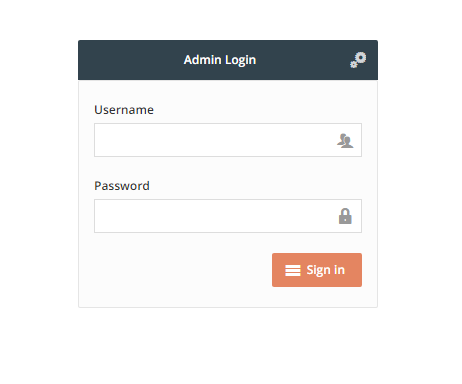
\includegraphics[scale=0.01]{Gambar/design-web/login}
}
\caption[Tampilan login]{Tampilan login} 
\label{fig:design_web_login}
\end{figure}

\begin{figure}
\centering
\resizebox{\textwidth}{!}{
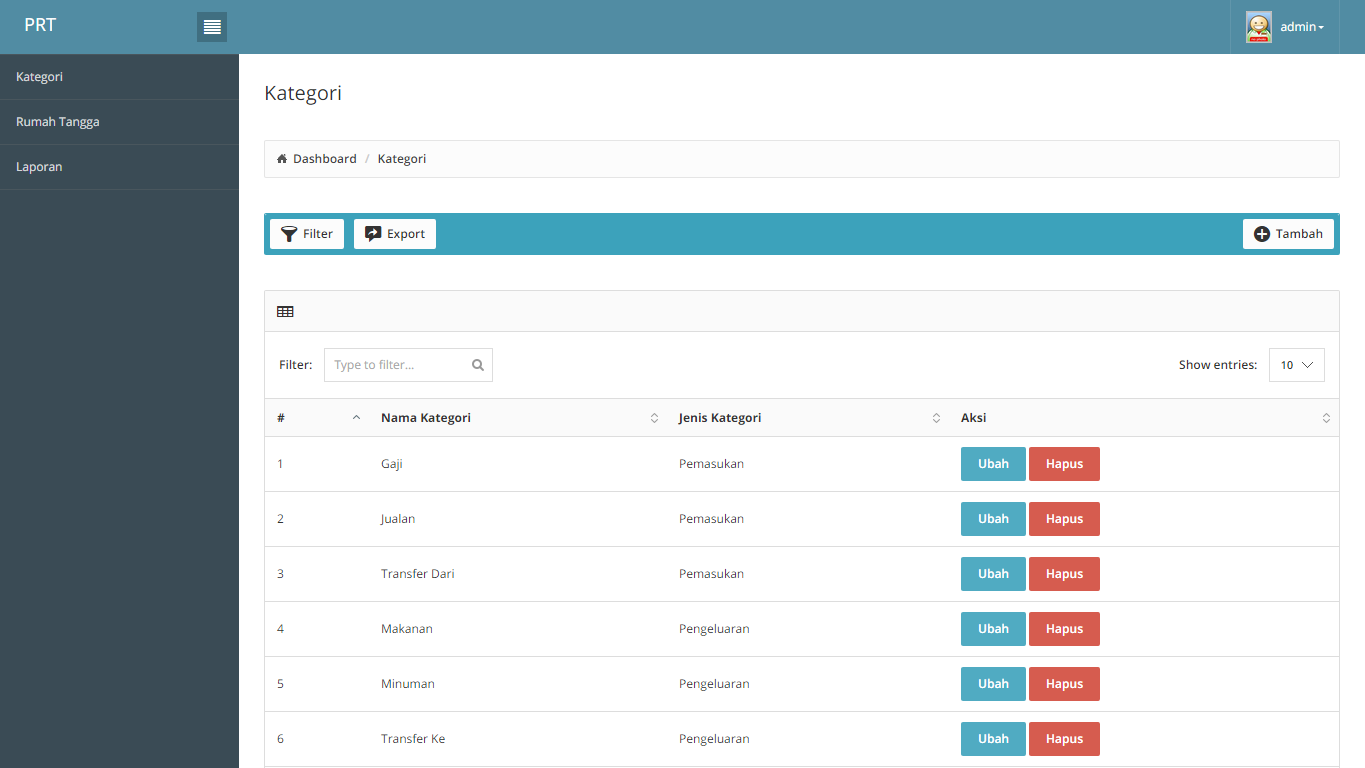
\includegraphics[scale=0.01]{Gambar/design-web/index_kategori}
}
\caption[Tampilan halaman kategori]{Tampilan halaman kategori} 
\label{fig:design_web_index_kategori}
\end{figure}

\begin{figure}
\centering
\resizebox{\textwidth}{!}{
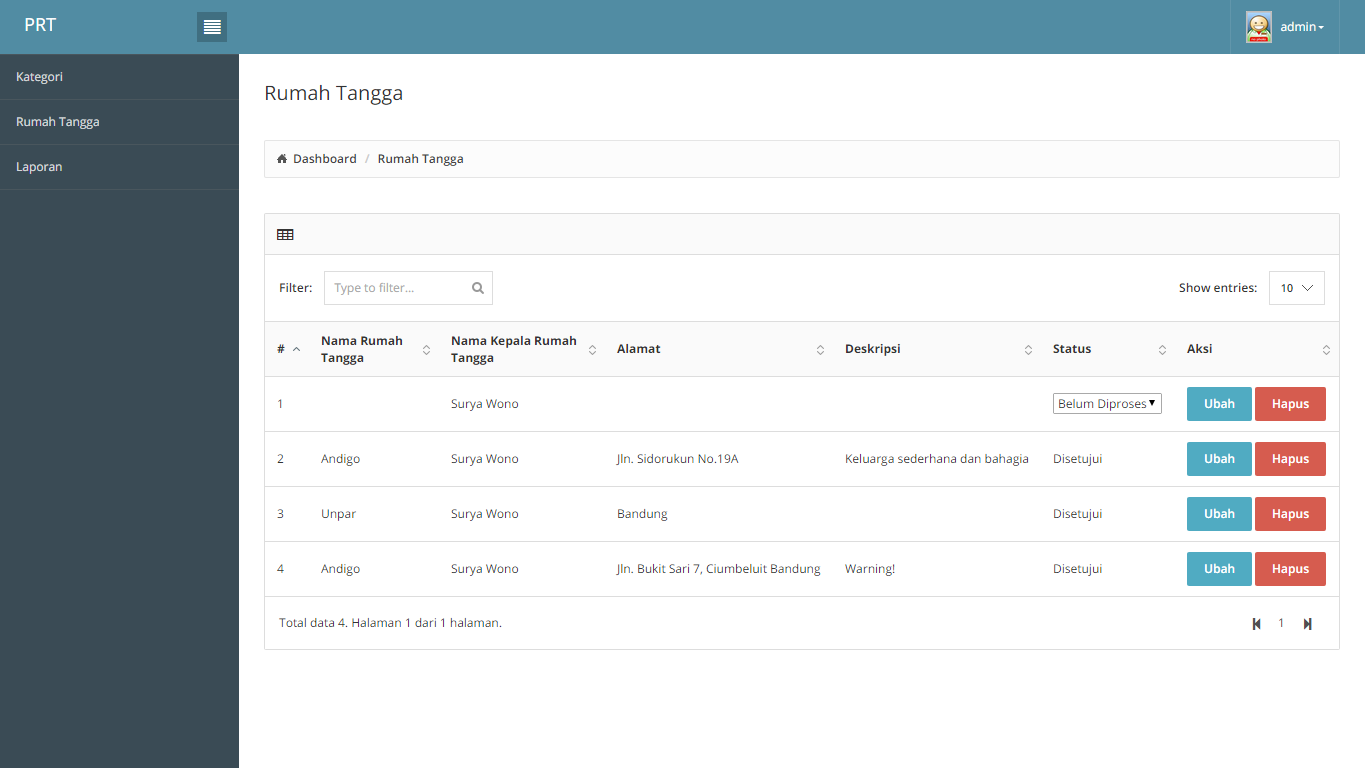
\includegraphics[scale=0.01]{Gambar/design-web/index_rumah_tangga}
}
\caption[Tampilan halaman rumah tangga]{Tampilan halaman rumah tangga} 
\label{fig:design_web_index_rumah_tangga}
\end{figure}

\section{Disain \textit{Webservice}}

\hspace{0,5cm}Pada webservice ini, terdapat dua peristiwa utama yaitu \textit{request} dan \textit{response}.Request akan memiliki beberapa parameter sesuai fungsi yang digunakan. Response yang dikembalikan dari \textit{webservice} berupan JSON dan memiliki format sesuai dengan Gambar~\ref{fig:format_response_webservice} dimana terdapat atribut utama yaitu \textit{response} yang membungkus tiga atribut lainnya yaitu status yang merupakan kode status dari \textit{request}, message yang merupakan keterangan status dan data yang merupakan atribut yang membungkus nilai-nilai yang dikembalikan.

\begin{figure}
\centering
\resizebox{\textwidth}{!}{
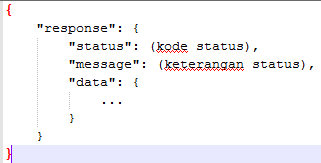
\includegraphics{Gambar/format_response_webservice}
}
\caption[Format \textit{response webservice}]{Format \textit{response webservice}} 
\label{fig:format_response_webservice}
\end{figure}

\textit{Request} dan \textit{response} pada \textit{webservice} untuk setiap fungsi akan dijelaskan sebagai berikut:
\begin{enumerate}
	\item Login (POST)
		\begin{itemize}
			\item Request pada Tabel~\ref{tab:request_login}
				\begin{table}[h]
					\centering
						\begin{tabular}{ |p{4cm}|p{10cm}|}
							\hline
							parameter & nilai \\ \hline
							email & email yang digunakan saat mendaftar \\ \hline
							password & password yang didaftarkan \\ \hline
					\end{tabular}
					\caption{\textit{Request login}}
					\label{tab:request_login}
				\end{table}
			\item Response pada Tabel~\ref{tab:response_login}
				\begin{table}[h]
					\centering
						\begin{tabular}{ |p{4cm}|p{10cm}|}
							\hline
							atribut & nilai \\ \hline
							status & 202 / 402 \\ \hline
							message & Login berhasil / Login gagal \\ \hline
							data & [data anggota dan rumah tangga] \\ \hline
						\end{tabular}
						\caption{\textit{Response login}}
					\label{tab:response_login}
				\end{table}
		\end{itemize}
		
		\item Menambah transaksi (POST)
		\begin{itemize}
			\item Request pada Tabel~\ref{tab:request_tambah_transaksi}
				\begin{table}[h]
					\centering
						\begin{tabular}{ |p{4cm}|p{10cm}|}
							\hline
							parameter & nilai \\ \hline
							kategori\_id & id kategori yang dipilih \\ \hline
							besaran & nilai transaksi \\ \hline
							deskripsi & deskripsi transaksi \\ \hline
							waktu & waktu transaksi \\ \hline
							anggota\_id & id anggota \\ \hline
					\end{tabular}
					\caption{\textit{Request} penambahan transaksi}
					\label{tab:request_tambah_transaksi}
				\end{table}
			\item Response pada Tabel~\ref{tab:response_tambah_transaksi}
				\begin{table}[h]
					\centering
						\begin{tabular}{ |p{4cm}|p{10cm}|}
							\hline
							atribut & nilai \\ \hline
							status & 200\\ \hline
							message & Berhasil disimpan \\ \hline
							data & [data sesuai request] \\ \hline
						\end{tabular}
						\caption{\textit{Request} penambahan transaksi}
					\label{tab:response_tambah_transaksi}
				\end{table}
		\end{itemize}
		
		\item Menyiapkan data laporan (GET)
		\begin{itemize}
			\item Request pada Tabel~\ref{tab:request_laporan}
				\begin{table}[h]
					\centering
						\begin{tabular}{ |p{4cm}|p{10cm}|}
							\hline
							parameter & nilai \\ \hline
							jenis & jenis laporan (tahun \& bulan) \\ \hline
							anggota\_id & id anggota \\ \hline
							tahun (untuk jenis bulanan) & tahun laporan \\ \hline
							bulan (untuk jenis mingguan) & minggu laporan \\ \hline
					\end{tabular}
					\caption{\textit{Request} penyiapan data laporan}
					\label{tab:request_laporan}
				\end{table}
			\item Response pada Tabel~\ref{tab:response_laporan}
				\begin{table}[h]
					\centering
						\begin{tabular}{ |p{4cm}|p{10cm}|}
							\hline
							atribut & nilai \\ \hline
							status & 400\\ \hline
							message & Data found \\ \hline
							data & [data laporan] \\ \hline
						\end{tabular}
						\caption{\textit{Response} penyiapan data laporan}
					\label{tab:response_laporan}
				\end{table}
		\end{itemize}
\end{enumerate}

\section{Disain Basis Data}
\label{sec:disainbasisdata}

\hspace{0,5cm}Pada sub-bab ini akan digambarkan disain basis data berupa \textit{Entity Relational Diagram} untuk aplikasi pembukuan rumah tangga dan \textit{website} pengolahan aplikasi pada Gambar~\ref{fig:er_diagram_prt}.

\begin{figure}[h]
\centering
\resizebox{\textwidth}{!}{
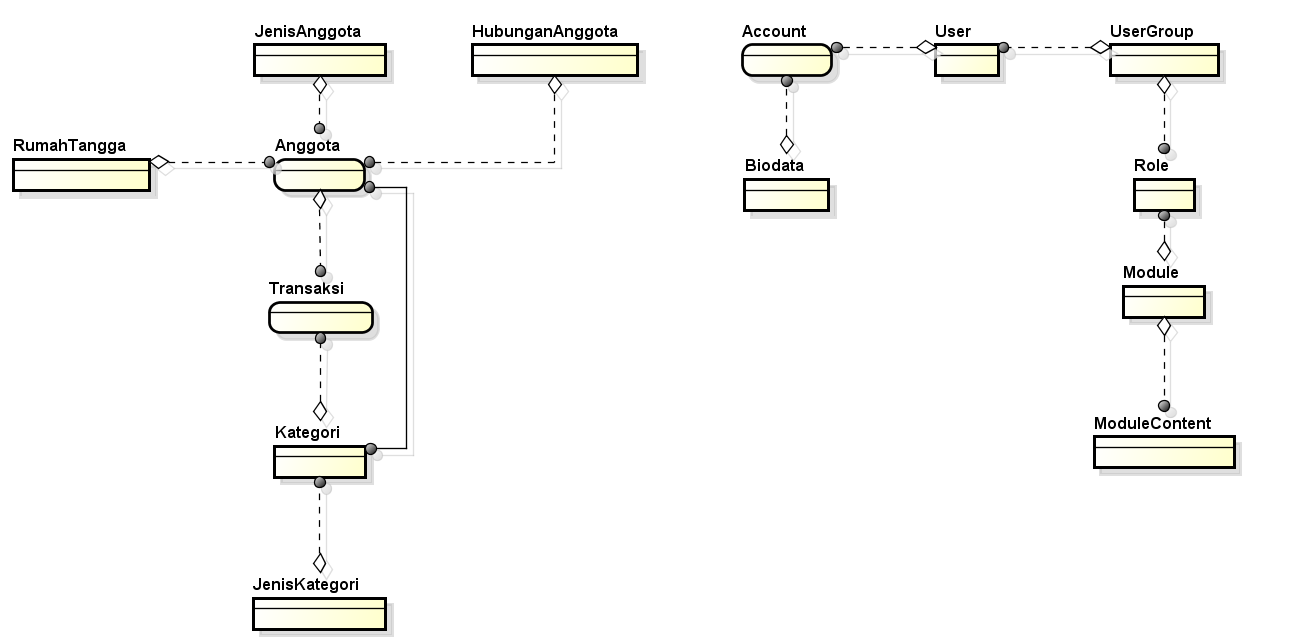
\includegraphics[scale=0.01]{Gambar/er-diagram}
}
\caption[\textit{Entity Relational Diagram} Pembukuan Rumah Tangga]{\textit{Entity Relational Diagram} Pembukuan Rumah Tangga} 
\label{fig:er_diagram_prt}
\end{figure}


}{}
\ifdefstring{\vbabe}{1}{\chapter{Introduction}
%\label{chap:intro}

\section{Motivation}
%%\label{sec:motivation}

A trajectory is the motion path of a moving object.
Various moving objects such as animals (probably in a wildlife area), hurricanes, or customers in a shopping area have trajectories that can provide valuable information.
For example, trajectory data can be used to predict the movement of the same type of object in similar situation in the future. 

During a tracking procedure, the location of these moving objects can be obtained using various location detection devices (e.g: RFID, GPS devices and mobile phones).
Later, this information will be sent to a database using any communication network (usually a wireless network).
Because typical trajectory data is obtained during a specific interval, then trajectory data also has a temporal component, besides its spatial component.

\begin{figure}
\centering
\includegraphics[scale=1]{Gambar/2d_trj}
\caption[Example of 2D trajectories with time component, from \cite{Vlachos:2002}]{Example of 2D trajectories with time component, from \cite{Vlachos:2002}} 
%\label{fig:2d_trj}
\end{figure}

The trajectory of a moving object is typically modeled as a sequence of consecutive locations in a multi-dimensional (generally two or three dimensional) Euclidean space \cite{Vlachos:2002}.
Figure~\ref{fig:2d_trj} shows an example of two trajectories from two objects which are moving in a 2D plane.
With their temporal component, we can see that these trajectories are represented as polylines in a 3D space.

Nowadays, with the rapid development of technologies in mobile computing and wireless communication, many devices with location acquisition capabilities make it possible to obtain huge volumes of trajectory data from various moving objects.
Furthermore, analysis of trajectory data is an important task for many applications that contain processing and managing moving objects, such as animal movements \cite{Calenge:2009,Nams:2004,Herb:2010,Brillinger:2001}, traffic and transport analysis \cite{Yunyao:1998}, defense and surveillance areas \cite{Ng:2001}, oceanographic observations\footnote{W.S. Kessler, ``Argo work in the coral sea.''http://faculty.washington.edu/kessler/noumea/gliders/\\argo\_coral\_sea.html, March 2010.}, weather and natural phenomena \cite{Hubert:1957}, people behavior \cite{Fuentes:2001} and sports \cite{Brillinger:2007,Iwase:2002}.

Previous work on trajectory data analysis shows that there are several ways to analyze sets of trajectories.
For example, similarity between trajectories can be determined \cite{VlachosGunopoulos:2002,Lin:2005,Kreveld:2007}.
Trajectories can also be clustered into groups with similar characteristics \cite{Gaffney:1999,Lee:2007,Nanni:2006,Buchin:2009}.
Other examples are common data mining tasks such as classification \cite{Lee:2008,Garcia:2006} and outlier detection \cite{LeeHan:2008}.
Furthermore, interesting movement patterns such as flocking can also be computed from a set of trajectories \cite{Gudmundsson:2006,Buchin:2008,Gudmundsson:2007,Laube:2006}.

Even though analysis and research on trajectories has expanded in recent years, several basic concepts still need to be studied further.
Some of them are the median and the mean trajectory for a collection/set of trajectories.
The median and the mean trajectory share some common properties: they should be similar to other trajectories in the set and all parts of them should be located roughly in the middle of the set.
However, there are several important differences between them:
Firstly, the median trajectory must use only parts of trajectories in the set. 
It uses only parts of one trajectory or combines parts from many different trajectories.
This property might be a disadvantage for the median because some parts of it can be located not in the middle of the set, but in several situations this might be useful.

Figure~\ref{fig:mean_dis} shows a set of four trajectories which avoid the light-blue obstacle.
The possible mean trajectory (the black trajectory in the right-hand side of the figure) will pass through the obstacle because the mean must lie in the middle of all trajectories in the set.
In this case, it is clear that the mean trajectory is not suitable for a path of a moving object.

The median trajectory (black trajectory in the left-hand side of the figure) gives a more suitable path because it always uses parts of other trajectories.
In parts near the obstacle, the median is not really in the middle of other trajectories.

\begin{figure}
\centering
\includegraphics[scale=1]{Gambar/mean_dis}
\caption[Example of the median (left) and the mean (right) trajectory \cite{Lionov:2009}]{Example of the median (left) and the mean (right) trajectory \cite{Lionov:2009}} 
%\label{fig:mean_dis}
\end{figure}

Secondly, the median trajectory is more robust against outliers than the mean trajectory.
Figure~\ref{fig:robust_med} shows this situation: we add one trajectory (with purple color) which can be categorized as an outlier compared to other trajectories. 
While the median trajectory only needs to be modified a little bit, the mean trajectory has to be changed a lot (comparing to the mean trajectory in Figure~\ref{fig:mean_dis}), to keep it in the middle of other trajectories.

\begin{figure}
\centering
\includegraphics[scale=1]{Gambar/robust_med}
\caption[Robustness of the median trajectory]{Robustness of the median trajectory} 
%\label{fig:robust_med}
\end{figure}

In this thesis, we will not cover the mean trajectory and only discuss the median trajectory and algorithms to compute it.
We also ignore the temporal component of the trajectory because it is not clear yet how to take it into account when computing the median trajectory. 
However, some research on motion and kinetic data structures contains a temporal component and are related to the median/mean trajectory \cite{Agarwal:2003,Agarwal:1997}. 

For other types of data, a median has a clear definition.
The median from a population (or a sample) of integer numbers is the number that separates the population into two halves, where at most half of the population have a smaller value and the other half of the population have a larger value than the median. 

For geometric data types, the concept of median also exist.
A \textit{center point} of a set $P$ of $n$ points in the plane is a point such that any closed half-plane whose bounding line contains the center point, contains at least $n/3$ points of $P$ \cite{Amenta:2000}.
If we force the center point to be one of the points from $P$, then we obtain a 2-dimensional version of the median, although the ``quality'' of this median can be bad.

The median trajectory does not have any formal definition yet.
Based on several properties that we mention earlier, such as its similarity with other trajectories and lying approximately in the middle of the set, we can determine a possible median, which can useful in several ways:

\subsection{Determine the most typical trajectory}
The property of the median trajectory makes it suitable to analyze the movement behavior or movement pattern from a group of same objects because the median somehow represents the whole trajectories in the set/collection.
The median trajectory properties, such as the length, the direction or the average speed (if we include the temporal component), could give valuable information.

Example applications include the detection of outliers, which can be done by analyzing the length and the similarity of the shape of the median with other trajectories.
Analyzing the average speed together with the shape of the median trajectory might be useful to understand the behavior and the movement pattern of people walking around in an area which has several interesting places to be visited (e.g., a zoo or an amusement park). 

\subsection{Better visualization for a set of trajectories}
Visualization of the median trajectory, together with its set of trajectories, might give the viewer a better interpretation and information about the set of trajectories.

\begin{figure}
\centering
\includegraphics[scale=1]{Gambar/all30_visual}
\caption[The set of 30 trajectories, starting at the blue point \& ending at the green point]{The set of 30 trajectories,starting at the blue point \& ending at the green point} 
%\label{fig:all30_visual}
\end{figure}

\begin{figure}
\centering
\includegraphics[scale=1]{Gambar/med_visual}
\caption[A set of 30 trajectories with its possible median trajectory]{A set of 30 trajectories with its possible median trajectory} 
%\label{fig:med_visual}
\end{figure}

We give an example in Figure~\ref{fig:all30_visual}, where a set has 30 trajectories, which is paths of 30 objects moving from the blue point to the green point.
From this figure, we can hardly tell anything about the general behavior or the direction of these trajectories. 
However, we know that several trajectories are different than others and probably can predict what the majority does, but it is still difficult to visualize what the majority of these trajectories does.

In the following figure (Figure~\ref{fig:med_visual}), we present a possible median trajectory as the red and thick trajectory.
From this visualization, it is clear what the majority of trajectories does.
Moreover, we can identify what parts of some trajectories are completely different from others. 

The visualization of the median trajectory could be useful in some real-life applications:
The median trajectory from trajectories of visitors in a national park can be used to see the most common path taken by visitors, which is probably the path that is preferred by future visitors.
This information might be useful if we want to create a map that can help those visitors by providing valuable information about a path and direction on that national park in the map, so that he/she can decide which path that he/she will take. 
% Other example is to use the median trajectory for video surveillance. 
% where median trajectory shows the most common path that the visitor take, and identify if there are any unusual trajectory

\subsection{\texorpdfstring{$k$}{k}-medoid clustering}
Another application that could use the median trajectory is the $k$-medoid algorithm, which is used in cluster analysis.
The $k$-medoid clustering algorithm is related to the $k$-means algorithm, a method to partition/group a set of objects into $k$ different clusters containing similar objects.

In general, each cluster in both algorithms has one object act as a \textit{central object} and other members of the cluster should be similar or having a small distance to this object.
The similarity or the distance between objects can be measured using different distance functions (e.g. Euclidean distance, Minkowski distance, etc), depending on the type of objects and the purpose of the clustering.

The main difference between the two algorithms is on the selection of the central object for each cluster. 
While the $k$-means simply uses the mean of objects, the $k$-medoid must use the medoid (an object which has the smallest average of dissimilarity/distance to all other objects in the set, but it must be a member of the set). 
This implies that $k$-means could create a new object to be the central object whereas the $k$-medoid must use one of the objects from the set.
Thus, the $k$-medoid algorithm is more suitable for spatial clustering purposes and less sensitive against noise and outliers.  

Partitioning Around Medoids (PAM) ~\cite{Kaufman:2005} is a basic $k$-medoid clustering algorithm.
It works as follow:
\begin{enumerate}
\item
Define a value $k$ and choose $k$ objects as a set of medoids.
\item
Assign every object to its closest/similar medoid and after that, compute the cost for the whole configuration.  
\item
Find another configuration by selecting a pair of medoid and non-medoid objects which have the smallest distance cost and swapping them temporarily.
Then, we assign all other objects to this temporary set of medoids and obtain a new configuration.
\item
If the new configuration has smaller cost than the last configuration, then we change the set of medoids and return to step 3
\item
Otherwise, stop and we find the set of medoids with their non-overlapping set of clusters.
\end{enumerate}

In case we want to cluster a set of trajectories, we can use the median trajectory as a medoid in this algorithm.
However, some changes probably should be made.
For example, finding another configuration is not done by simply swapping the median with other trajectory, instead we can choose to swap part of them (with the requirement that both trajectories intersect one another).

\section{Basic Idea of the Research}
%\label{sec:basic_idea}

Consider a set $T$ of $m$ trajectories.
We want to to compute the median trajectory of $T$.
In this set, all trajectories have the same start and end points.
The median trajectory of $T$ must be built using parts of trajectories in $T$ and somehow must follow what other trajectories in $T$ do, while staying in the ``middle'' of other trajectories.

\subsection{The Simple Switching Method }
%\label{sec:switch}

A simple idea to obtain a median trajectory from $T$ is to start from the ``middle'' trajectory, which is the $(m+1)/2$-level of arrangement formed by all trajectories in $T$ (we assume $m$ is odd).
At every intersection point, the median trajectory will switch to another trajectory and keep $(m+1)/2$ trajectories above and below the median \cite{Buchin:2010}.

\begin{figure}
\centering
\includegraphics[scale=1]{Gambar/switch_fail0}
\caption[Illustration of the simple idea using switching]{Illustration of the simple idea using switching} 
%\label{fig:switch_fail0}
\end{figure}

\begin{figure}
\centering
\includegraphics[scale=1]{Gambar/switch_fail1}
\caption[The median trajectory make a shortcut path \cite{Lionov:2009}]{The median trajectory makes a shortcut \cite{Lionov:2009}} 
%\label{fig:switch_fail1}
\end{figure} 

Figure~\ref{fig:switch_fail0} shows the result (the median trajectory is the thick-blue trajectory) of this approach for two different types of set of trajectories, one of them contains trajectories with self intersection.
From the right-hand side of the figure in Figure~\ref{fig:switch_fail0}, we can see that this method cannot produce suitable median trajectory because the median does not follow the loop created by the three trajectories.

In general, this method will not give a suitable median if a set of trajectories contains self-intersecting trajectories.
More examples from \cite{Lionov:2009} show several ``incorrect'' median trajectories obtained by using this simple switching method.
The blue median trajectory in Figure~\ref{fig:switch_fail1} makes a shortcut path to the end point.

\begin{figure}
\centering
\includegraphics[scale=1]{Gambar/switch_fail2}
\caption[The median trajectory does not stay in the middle \cite{Lionov:2009}]{The median trajectory does not stay in the middle \cite{Lionov:2009}} 
%\label{fig:switch_fail2}
\end{figure} 

The median trajectory in Figure~\ref{fig:switch_fail2} does not stay in the "middle" of other trajectories.
Finally, in Figure~\ref{fig:switch_fail3}, the median trajectory does not follow the sequence of regions as the other trajectories. 
The correct sequence of regions is $1-2-3-4-5-6-7-8$.

\begin{figure}
\centering
\includegraphics[scale=1]{Gambar/switch_fail3}
\caption[The median trajectory follows incorrect direction \cite{Lionov:2009}]{The median trajectory does not follow the correct sequence of regions \cite{Lionov:2009}} 
%\label{fig:switch_fail3}
\end{figure} 
 
\subsection{The Algorithm Using the Concept of Homotopy}
%\label{sec:homotopy}

Another algorithm to compute the median trajectory uses the concept of homotopy (along with the modified simple switching method) \cite{Buchin:2010}.
This algorithm works by placing cross in a relatively large face bounded by segments from a set of trajectories.
Figure~\ref{fig:homotopy} shows an example where cross is placed in the relatively large bounded face and two crosses are placed in the outer face.

\begin{figure}
\centering
\includegraphics[scale=1]{Gambar/homotopy}
\caption[Illustration of the algorithm using homotopy concept]{Illustration of the algorithm using homotopy concept} 
%\label{fig:homotopy}
\end{figure}

Based on the location of these crosses, each trajectory in $T$ will be assigned a \textit{signature}.
Figure~\ref{fig:base_sign} shows three trajectories and two crosses \textit{a} and \textit{b}. 
From these two crosses, four half-lines are created: \textit{$a^{+}$} and \textit{$a^{-}$} are half-lines above and below \textit{a}, while \textit{$b^{+}$} and \textit{$b^{-}$} are half-lines above and below \textit{b}, respectively. 

For all trajectories in $T$, we give them a signature based on how they intersect with the half-line(s) from the crosses. 
Note that each trajectory might have a different signature, because it depends on the position of the trajectory with respect to all crosses in the plane.
In Figure~\ref{fig:base_sign}, the blue trajectory intersect with \textit{$a^{-}$} and \textit{$b^{+}$}, thus its signature will be \textit{$a^{-}b^{+}$} (the order is following the direction of the trajectory). 
In the same way, the signature of the red trajectory will be the same as the green trajectory: \textit{$a^{-}b^{-}$}.

\begin{figure}
\centering
\includegraphics[scale=1]{Gambar/base_sign}
\caption[Trajectories and crosses]{Trajectories and crosses} 
%\label{fig:base_sign}
\end{figure}

% The next step of the algorithm is to create the subset $T'$ of $T$.
% All trajectories in $T'$ must be homotopic to each other and also the set with the most number of trajectories from $T$.

Two different trajectories are homotopic if one trajectory can be deformed continuously into the other one without passing through any crosses, while the start and end point are not moved.
Naturally, two trajectories are homotopically equivalent if their signatures are exactly the same. 
However, two homotopic trajectories do not always have the same signatures.
We shown an example in Figure~\ref{fig:diff_sign} where the blue and the black trajectory are homotopic, but their signatures are different.

To determine whether two trajectories with different signature are homotopic or not, we perform a \textit{reduce} operation.
This \textit{reduce} operation works by eliminating two exact same signs, if their position is next to each other in the signature.
In Figure~\ref{fig:diff_sign}, the signature of the blue trajectory is \textit{$a^{-}b^{+}c^{+}c^{+}b^{+}b^{-}c^{-}$}.
Notice that it has two \textit{$c^{+}$} that we can eliminate.
This will change the signature of the blue trajectory into \textit{$a^{-}b^{+}b^{+}b^{-}c^{-}$}.
Once again, we can identify that two \textit{$b^{+}$} are positioned directly to each other. 
Performing the reduce operation again, we will get the final signature of the blue trajectory: \textit{$a^{-}b^{-}c^{-}$}.
At this point, we cannot apply the reduce operation again to this signature, and we say that the signature has been \textit{maximally reduced}.
Finally,we conclude that if two trajectories have the same maximally reduced signature, then the two trajectories are homotopically equivalent.  

\begin{figure}
\centering
\includegraphics[scale=1]{Gambar/diff_sign}
\caption[The blue and black trajectory are homotopically equivalent \cite{Lionov:2009}]{The blue and black trajectory are homotopically equivalent \cite{Lionov:2009}} 
%\label{fig:diff_sign}
\end{figure}

The next step of the algorithm is to create a subset $T'$ of $T$, and then find the median trajectory by using only parts of trajectories from $T'$.
Creating $T'$ is straightforward, we only need to compute maximally reduced signature for all trajectories and choose a subset with the largest number of trajectories which have the same signature.

To create the median trajectory from $T'$, we use the modified version of the switching method.
This method start at the first segment of the``middle'' trajectory.
We find such a segment by determine the outer face of the set of trajectories.
The first segment of the ``middle'' trajectory is the segment where there are $(n-1)/2$ first segments from other trajectories (assume $n$ is odd) between the segment and the outer face (on each side of the segment).
% The algorithm starts with the trajectory which $(n-1)/2$ trajectories in $T'$ are above and the rest are below it (assume $n$ is odd).


Then, at every intersection, the median will switch to another trajectory if the continuation along this trajectory (without ever switching again) gives the same signature with the signature of one trajectory from $T'$.
Figure~\ref{fig:homotopy_algo} shows an example of this algorithm.
After starting with the red trajectory and switching to the green trajectory at the first intersection, the next intersection is with the blue trajectory (at the small blue square) and so far, the signature for the median is \textit{$a^{+}$}. 
Although the blue trajectory is going forward, the signature after this intersection while following the blue trajectory (until the end point) is \textit{$b^{-}c^{-}$}. 

\begin{figure}
\centering
\includegraphics[scale=1]{Gambar/hmtp_works}
\caption[Modified switching method \cite{Lionov:2009}]{Modified switching method \cite{Lionov:2009}} 
%\label{fig:homotopy_algo}
\end{figure}

If the median switches at this intersection, the final signature will be \textit{$a^{+}b^{-}c^{-}$}, which is not the signature of this set (\textit{$a^{+}b^{-}b^{+}b^{-}c^{-}$}). 
At this point, the median does not switch to another trajectory. 
Instead, it continues to move along the green trajectory. 
The same situation also occurs when the median (now following the blue trajectory) intersects with the green trajectory (at the small green square).

Although this algorithm can produce a more suitable median trajectory for the situation where the switching method fails, the quality of the homotopic median trajectory depends heavily on the following factors:
\begin{itemize}
\item placement of the crosses
\item the number of trajectories which have the same signature 
\end{itemize}

Therefore, in several cases the algorithm with the homotopy concept cannot produce suitable median trajectories.
We give two examples in Figure~\ref{fig:homotopy_fail0}: in the left-hand side of figure, the final median trajectory (blue) does not follow other trajectories to the area with a narrow space. 
This problem arises because that narrow space is not large enough for a cross to be placed. 

\begin{figure}
\centering
\includegraphics[scale=1]{Gambar/homotopy_fail0}
\caption[Example cases where algorithm using homotopy will fail]{Example cases where algorithm using homotopy will fail} 
%\label{fig:homotopy_fail0}
\end{figure}

In the right-hand side of the figure, there are no two trajectories homotopically equivalent to each other. 
Nevertheless, by looking at their position, the median trajectory should be the one in the middle (between the two crosses).
However, the algorithm with the homotopy concept does not guarantee that a suitable median trajectory will be found because there is no subset that contains the majority of trajectories in $T$. 
Figure~\ref{fig:homotopy_fail1} shows an example from \cite{Lionov:2009}, where the median trajectory does not completely follow what other trajectories do.

\begin{figure}
\centering
\includegraphics[scale=1]{Gambar/homotopy_fail1}
% \caption[The median trajectory does not pass through part of trajectories in the upper left area]{The median trajectory does not pass through part of trajectories in the upper left area} 
\caption{The median trajectory does not pass through part of trajectories in the upper left area}
%\label{fig:homotopy_fail1}
\end{figure}

\subsection{The Proposed Solutions}
%\label{sec:solution}

To solve the problems we mention in the previous section, we propose two algorithms to compute the median trajectory from a set of $m$ trajectories (where each trajectory has $n$ segments).

The first algorithm is an $O(1.2108^{m} + m^{5}n^{5})$ worst-case time algorithm.
This algorithm uses the Fr\'{e}chet Distance \cite{AltGodau:1995} and works similar to the algorithm using the homotopy concept because both of them have to create the largest subset of similar trajectories and then compute the median trajectory by using parts of trajectories in that subset. 
By using the Fr\'{e}chet Distance, we avoid the requirement to find proper places to put crosses, but still can produce suitable median trajectory in the situation where the homotopic algorithm fails (e.g. the example with a narrow space).

The second algorithm uses the combination of the buffer concept and Dijkstra's Shortest Path algorithm.
Unlike all previous algorithms, this algorithm does not need to find the largest subset consisting similar trajectories. 
% Thus, it will solve the second problem from the homotopy concept, where each trajectory is different from each other .
Using this algorithm, we can compute the median trajectory in $O(h^{2} \log h)$ time in the worst-case, where $h$ is the number of all segments in $T$ $(h = O(mn))$.

We implemented the second algorithm in Java programming language and experiments have been done to determine the quality of the resulting median trajectory produced by this algorithm.
To provide the test data (set of trajectories), we use a trajectories generator instead of using real-world data.
This allow us to test much larger sets of trajectories

\section{Outline of the Thesis}
%\label{sec:outline}

Chapter 2 describes the properties for a set of trajectories and also some properties the median trajectory should have.

The next two chapters explain in detail the two algorithms:
\begin{itemize}
\item 
Chapter 3 starts with a brief introduction of the Fr\'{e}chet Distance and after that, we will explain how to use it to compute the median trajectory. 
\item 
Chapter 4 introduces the method to compute the median trajectory using the combination of the buffer concept and Dijkstra's shortest path algorithm. 
\end{itemize}

We will give an explanation about our implementation, particularly on the implementation of the trajectories generator, in Chapter 5.
In Chapter 6, we present the measures used to evaluate the quality of the median trajectory, the experiments set-up and the results from the experiments.
This thesis will be concluded in Chapter 7 and 8, where we draw conclusions and discuss some issues and possible directions for further research.

\lipsum[1-14]}{}
\ifdefstring{\vbabf}{1}{\include{Bab/bab6}}{}
%\ifdefstring{\vbabg}{1}{\include{Bab/bab7}}{}
%\ifdefstring{\vbabh}{1}{\include{Bab/bab8}}{}
%\ifdefstring{\vbabi}{1}{\include{Bab/bab9}}{}

\bibliographystyle{ieeetr}
\bibliography{pustaka}

\appendix
\apptoc

\tampillmp{\vlmp}
\ifdefstring{\vlmpa}{1}{\chapter{Form Survey}
\label{app:A}
\includepdf[pages={1,2}]{Gambar/survey.pdf}}{}
\ifdefstring{\vlmpb}{1}{\chapter{Hasil Survey}
\label{app:B}
\includepdf[pages={1,2}]{Gambar/hasil_survey.pdf}}{}
\ifdefstring{\vlmpc}{1}{\include{Lampiran/lampC}}{}
\ifdefstring{\vlmpd}{1}{\include{Lampiran/lampD}}{}
\ifdefstring{\vlmpe}{1}{\include{Lampiran/lampE}}{}
\ifdefstring{\vlmpf}{1}{\include{Lampiran/lampF}}{}
\ifdefstring{\vlmpg}{1}{\include{Lampiran/lampG}}{}
\ifdefstring{\vlmph}{1}{\include{Lampiran/lampH}}{}
\ifdefstring{\vlmpi}{1}{\include{Lampiran/lampI}}{}

\end{document}
